\documentclass{book}

% Configuration
% ------------------
% Packages
% ------------------
\usepackage[export]{adjustbox}
\usepackage[english]{babel}
\usepackage[T1]{fontenc}
\usepackage[scaled]{helvet}
\usepackage[utf8]{inputenc}
\usepackage[letterpaper,top=1in,bottom=1in,inner=1.25in,outer=1in]{geometry}
\usepackage[dvipsnames]{xcolor}

\usepackage{algorithm}
\usepackage{algorithmicx}
\usepackage{algpseudocode}
\usepackage{amsfonts,amsmath,amsthm,amssymb}
\usepackage{booktabs}
\usepackage{etoolbox}
\usepackage{float}
\usepackage{graphicx}
\usepackage{latexsym}
\usepackage{mathtools}
\usepackage{sectsty}
\usepackage{setspace}
\usepackage{subcaption}
\usepackage{tabularx}
\usepackage{tikz}
% \usepackage{txfonts}
\usepackage{url}
\usepackage{wrapfig}
\usepackage{xparse}


% ------------------
% Shortcuts
% ------------------
\newcommand{\floor}[1]{\lfloor #1 \rfloor}
\newcommand{\ceil}[1]{\lceil #1\rceil}

\newcommand{\bigo}[1]{\ensuremath{\mathcal{O}\left(#1\right)}}

\usetikzlibrary{decorations.pathmorphing}
\newcommand{\zigzagarrow}{
    \tikz{
        \draw[->, decorate, decoration={zigzag, segment length=4, amplitude=.9, post=lineto, post length=2pt}] (0,0) -- (0.5,0);
    }
}

\newcommand{\R}{\mathbb{R}}

\newcommand{\blue}[1]{{\color{blue}#1}}
\newcommand{\red}[1]{{\color{red}#1}}

% ------------------
% Command Redefinitions
% ------------------
\renewcommand{\qed}{\hfill$\blacksquare$}

\makeatletter
\renewcommand*\env@matrix[1][*\c@MaxMatrixCols c]{%
    \hskip -\arraycolsep
    \let\@ifnextchar\new@ifnextchar
    \array{#1}}
\makeatother

\algrenewcommand\algorithmicfunction{\textsc{\color{primary}Function}}
\algrenewcommand\algorithmicif{\textsc{\color{primary}If}}
\algrenewcommand\algorithmicelse{\textsc{\color{primary}Else}}
\algrenewcommand\algorithmicreturn{\textsc{\color{primary}Return}}
\algrenewcommand\algorithmicwhile{\textsc{\color{primary}While}}
\algrenewcommand\algorithmicfor{\textsc{\color{primary}For}}

\algrenewcommand\Call[2]{\textproc{\color{primary}\textsc{#1}}(#2)}

\newcommand{\To}{\textsc{\color{primary}To}\xspace}

\algtext*{EndIf}
\algtext*{EndWhile}
\algtext*{EndFor}
\algtext*{EndFunction}

% ------------------
% Colors
% ------------------
\definecolor{primary}{HTML}{207BA5}
\definecolor{greybg}{RGB}{249, 249, 249}

\definecolor{thmbg}{HTML}{F2F2F9}
\definecolor{lemmabg}{HTML}{FFFAF8}
\definecolor{lemmafr}{HTML}{983b0f}
\definecolor{propbg}{HTML}{f2fbfc}
\definecolor{propfr}{HTML}{191971}
\definecolor{myp}{RGB}{197, 92, 212}
\definecolor{grey17}{RGB}{17, 17, 17}
\definecolor{MyGrey}{HTML}{5B5B5B}

\definecolor{lightBlue}{rgb}{0.0, 0.64, 1.0}
\definecolor{lightRed}{rgb}{1.0, 0.50, 0.50}
\definecolor{darkGreen}{rgb}{0.31, 0.54, 0.30}
\definecolor{violet}{RGB}{186, 153, 242}
\definecolor{darkRed}{HTML}{BF0813}

%----------------
%	Text Styles
%----------------
\DeclareTextFontCommand{\term}{\color{orange}\bfseries}
\DeclareTextFontCommand{\bred}{\color{darkRed}\bfseries}
\DeclareTextFontCommand{\itblue}{\color{lightBlue}\itshape}

\DeclareTextFontCommand{\vector}{\bfseries\itshape}

% ------------------
%   URL Color
% ------------------
\usepackage[colorlinks=true]{hyperref}
\hypersetup{
    colorlinks=true,
    linkcolor=black,
    filecolor=magenta,
    urlcolor=blue,
}

% ------------------
% Tikz Externalize
% ------------------
\usetikzlibrary{external}
\tikzexternalize[prefix=tikz/]
% Disable externalization globally, and only enable it for `tikzpicture'
\tikzexternaldisable
\BeforeBeginEnvironment[label]{tikzpicture}{\tikzexternalenable}
\AfterEndEnvironment[label]{tikzpicture}{\tikzexternaldisable}

% ------------------
% Boxes
% ------------------
\usepackage[most]{tcolorbox}

\newcommand\fancybox[3]{%
    \tcbset{
        mybox/.style={
                enhanced,
                boxsep=0mm,
                opacityfill=0,
                overlay={
                        \coordinate (X) at ([xshift=-1mm, yshift=-1.5mm]frame.north west);
                        \node[align=right, text=#1, text width=2.5cm, anchor=north east] at (X) {\bf#2};
                        \draw[line width=0.5mm, color=#1] (frame.north west) -- (frame.south west);
                    }
            }
    }
    \begin{tcolorbox}[mybox]
        #3
    \end{tcolorbox}
}

\tcbuselibrary{theorems,skins,hooks}
\NewDocumentCommand\thmbox{m O{\Large #1} O{greybg} O{primary} O{number within=section}}
{
    \newtcbtheorem[#5]{#1}{\large #2}
    {%
        enhanced,
        breakable,
        colback = #3,
        frame hidden,
        boxrule = 0sp,
        borderline west = {2pt}{0pt}{#4},
        sharp corners,
        detach title,
        before upper = \tcbtitle\par\smallskip,
        coltitle = #4,
        fonttitle = \bfseries,
        %description font = \mdseries,
        separator sign none,
        segmentation style={solid, #4}
    }
    {th}
}

\thmbox{Corollary}[Corollary][myp!10][myp!85!black]
\thmbox{Lemma}[Lemma][lemmabg][lemmafr]
\thmbox{Propo}[Proposition][propbg][propfr]
\thmbox{Defi}[Definition][primary!12][primary]
\thmbox{Notation}[Notation][white][grey17][no counter]
\thmbox{Theorem}[Theorem][primary!12][primary]
\thmbox{Remark}[Remark][grey17!10][grey17][no counter]

% ------------------
% Environments
% ------------------
\newenvironment{corollary}[1][]   {\begin{Corollary}{#1}{}}                               {\end{Corollary}}
\newenvironment{definition}[1][]  {\begin{Defi}{#1}{}}                                    {\end{Defi}}
\newenvironment{lemma}[1][]       {\begin{Lemma}{#1}{}}                                   {\end{Lemma}}
\newenvironment{lemma*}[1][]      {\begin{Lemma*}{#1}{}}                                  {\end{Lemma*}}
\newenvironment{proposition}[1][] {\begin{Propo}{#1}{}}                                   {\end{Propo}}
\newenvironment{remark}[1][]      {\begin{Remark}{#1}{}}                                  {\end{Remark}}
\newenvironment{theorem}[1][]     {\begin{Theorem}{#1}{}}                                 {\end{Theorem}}

\newenvironment{rtheorem}[2][]    {\begin{Theorem}{#1}{#2}}                               {\end{Theorem}}

\theoremstyle{definition}
\newtheorem*{exam}{\color{primary}Example}
% \newcommand{\example}[1]{\begin{exam}#1\end{exam}}
% \newenvironment{example}          {\begin{exam}} {\begin{flushright}${\color{primary}\diamondsuit}$\end{flushright} \end{exam}}
\newenvironment{example}          {\begin{exam}} {\hfill${\color{primary}\diamondsuit}$\end{exam}}

\theoremstyle{definition}
\newtheorem*{clm}{\color{MyGrey}Claim}
\newenvironment{claim}            {\begin{clm}} {\end{clm}}

% ------------------
% Lists
% ------------------
\usepackage{enumitem}

\newcommand{\cnumero}[2]{
    \tikz[baseline=(char.base)]
    \node[minimum size=0.2cm,circle,inner sep=1pt,draw, #2,thick,fill=#2](char)
    {\color{white}\bfseries\fontsize{8}{8}#1};}
\newcommand*{\itembolasazules}[1]{\protect\cnumero{#1}{primary}}

% \newenvironment{listo} {\begin{enumerate}[label=\itembolasazules{\arabic*}]} {\end{enumerate}}
% \newenvironment{listu} {\begin{itemize}  [label=$\color{primary} \bullet$]}  {\end{itemize}}

\setlist[itemize]{label=$\color{primary} \bullet$}
\setlist[enumerate]{label=\itembolasazules{\arabic*}}

% ------------------
% Table of Contents
% ------------------
\usepackage{blindtext}
\usepackage{framed}
\usepackage{titletoc}

\patchcmd{\tableofcontents}{\contentsname}{\contentsname}{}{}

\renewenvironment{leftbar}
{\def\FrameCommand{\hspace{6em}%
        {\color{primary}\vrule width 2pt depth 6pt}\hspace{1em}}%
    \MakeFramed{\parshape 1 0cm \dimexpr\textwidth-6em\relax\FrameRestore}\vskip2pt%
}
{\endMakeFramed}

\titlecontents{chapter}[0em]
{\vspace*{2\baselineskip}}
{\parbox{4.5em}{%
        \hfill\Huge\bfseries\color{primary}\thecontentslabel}%
    \vspace*{-2.3\baselineskip}\leftbar\textbf{\color{primary}\small\chaptername~\thecontentslabel}\\
}{}{\endleftbar}

\titlecontents{section}[8.4em]
{\contentslabel{3em}}{}{}
{\hspace{0.5em}\nobreak\itshape\color{primary}\contentspage}

\titlecontents{subsection}[11.4em]
{\contentslabel{3em}}{}{}
{\hspace{0.5em}\nobreak\itshape\color{primary}\contentspage}

% ------------------
% Chapters
% ------------------
\newtcolorbox{titlecolorbox}[1]{ %the box around chapter
    coltext=white,
    colframe=primary,
    colback=primary,
    boxrule=0pt,
    arc=0pt,
    notitle,
    width=4.8em,
    height=2.4ex,
    before=\hfill
}

\usepackage[explicit]{titlesec}

\makeatletter
\let\old@rule\@rule
\def\@rule[#1]#2#3{\textcolor{primary}{\old@rule[#1]{#2}{#3}}}
\makeatother

\titleformat{\chapter}[display]
{\Huge}
{}
{0pt}
{\begin{titlecolorbox}{}
        {\large\MakeUppercase{\bf\chaptername}}
    \end{titlecolorbox}
    \vspace*{-3.19ex}\noindent\rule{\textwidth}{0.4pt}
    \parbox[b]{\dimexpr\textwidth-4.8em\relax}{\raggedright\MakeUppercase{#1}}{\hfill\fontsize{70}{60}\selectfont{\color{primary}\thechapter}}
}
[]

\titleformat{name=\chapter,numberless}[display]
{\Huge}
{}
{0pt}
{
    \vspace*{-3.19ex}\noindent\rule{\textwidth}{0.4pt}
    \parbox[b]{\dimexpr\textwidth-4.8em\relax}{\raggedright\MakeUppercase{#1}}
}
[]

% ------------------
% Sections
% ------------------
\titleformat{\section}[hang]{\Large\bfseries}%
{\rlap{\color{primary}\rule[-6pt]{\textwidth}{0.4pt}}\colorbox{primary}{%
        \raisebox{0pt}[13pt][3pt]{ \makebox[60pt]{% height, width
                \selectfont\color{white}{\thesection}}
        }}}%
{15pt}%
{ \color{primary}#1
    %
}
\titlespacing*{\section}{0pt}{3mm}{5mm}
% ------------------
% Subsections
% ------------------
\subsectionfont{\Large\color{primary}}

% ------------------
% Bibliography and Index
% ------------------
\usepackage{csquotes}
\usepackage[
    style=ieee, 
    citestyle=ieee,
    sorting=nyt,
    sortcites=true,
    autopunct=true,
    autolang=hyphen,
    hyperref=true,
    abbreviate=false,
    backref=true,
    backend=biber,
    defernumbers=true
]{biblatex}
\addbibresource{./bibliography.bib} % BibTeX bibliography file
\defbibheading{bibempty}{}

\usepackage{calc} % For simpler calculation - used for spacing the index letter headings correctly
\usepackage{makeidx} % Required to make an index
\makeindex % Tells LaTeX to create the files required for indexing

% ------------------
% Title page
% ------------------
\usetikzlibrary{calc}
\usetikzlibrary{shapes.geometric}
\usepackage{anyfontsize}
\newcommand{\frontpage}[3]{
    \tikzset{external/export next=false}
    \begin{tikzpicture}[remember picture, overlay]
        % Background
        \fill[primary] (current page.south west) rectangle (current page.north east);

        \foreach \i in {2.5,...,22} {
            \node[rounded corners,primary!60,draw,regular polygon,regular polygon sides=6, minimum size=\i cm,ultra thick] at ($(current page.west)+(2.5,-5)$) {} ;
        }

        % Background Polygon
        \foreach \i in {0.5,...,22} {
            \node[rounded corners,primary!60,draw,regular polygon,regular polygon sides=6, minimum size=\i cm,ultra thick] at ($(current page.north west)+(2.5,0)$) {} ;
        }

        \foreach \i in {0.5,...,22} {
            \node[rounded corners,primary!90,draw,regular polygon,regular polygon sides=6, minimum size=\i cm,ultra thick] at ($(current page.north east)+(0,-9.5)$) {} ;
        }

        \foreach \i in {21,...,6} {
            \node[primary!85,rounded corners,draw,regular polygon,regular polygon sides=6, minimum size=\i cm,ultra thick] at ($(current page.south east)+(-0.2,-0.45)$) {} ;
        }

        % Title
        \node[left,primary!5,minimum width=0.625*\paperwidth,minimum height=3cm, rounded corners] at ($(current page.north east)+(0,-9.5)$) {
            {\fontsize{25}{30} \selectfont \bfseries #1}
        };

        % Subtitle
        \node[left,primary!10,minimum width=0.625*\paperwidth,minimum height=2cm, rounded corners] at ($(current page.north east)+(0,-11)$) {
            {\huge \textit{#2}}
        };

        % Author
        \node[left,primary!5,minimum width=0.625*\paperwidth,minimum height=2cm, rounded corners] at ($(current page.north east)+(0,-13)$) {
            {\Large \textsc{#3}}
        };

        % Year
        \node[rounded corners,fill=primary!70,text =primary!5,regular polygon,regular polygon sides=6, minimum size=2.5 cm,inner sep=0,ultra thick] at ($(current page.west)+(2.5,-5)$) {\LARGE \bfseries \the\year{}};
    \end{tikzpicture}
}


\begin{document}

\pagestyle{empty}
\frontpage{CSC373}{Algorithm Design, Analysis \& Complexity}{Sinan Li}
\newpage

\tableofcontents
\newpage

\tikzset{
    graph-node/.style={
        circle,
        fill=red,
        draw=black,
        line width=0.5pt,
        inner sep=1.5pt
    },
    every edge/.style={
        draw,
        thick,
    },
    non-edge/.style={
        dotted,
        lightBlue,
    },
}

% No indent
\setlength{\parindent}{0pt}

\part{Notes}

\chapter{Introduction}

\section{Course Information}

\begin{itemize}
    \item \textbf{Instructor}: Nathan Wiebe

    \begin{itemize}
        \item \textbf{Email}: \href{mailto:nawibe@cs.toronto.edu}{nawibe@cs.toronto.edu}
        \item \textbf{Office}: SF 3318C
    \end{itemize}

    \item \textbf{Text}: [CLRS] \textit{Introduction to Algorithms}: Cormen, Thomas H., Leiserson, Charles E., Rivest, Ronald L., Stein, Clifford

    % Optional: 
    
    % \begin{itemize}
    %     \item [DPV] \textit{Algorithms}: Dasgupta, Sanjoy, Papadimitriou, Christos H., Vazirani, Umesh
    %     \item [KT] \textit{Algorithm Design}: Kleinberg, Jon, Tardos, Eva
    % \end{itemize}

    \item \textbf{Disclaimer}: Many things are up in the air, so expect a somewhat bumpy ride at the start but hopefully, we will get through together! Use any of the feedback mediums (email, Piazza, \dots) to let the instructor know if there are any suggestions for improvement. 
\end{itemize}

\section{Grading}

\subsection{Assignments}

\begin{itemize}
    \item \bred{4 assignments}, best 3 out of 4
    \item Group work
    \begin{itemize}
        \item In groups of \itblue{up to three} students
        \item Best way to learn is for each member to try each problem
    \end{itemize}
    \item Questions will be \bred{more difficult}
    \begin{itemize}
        \item May need to mull them over for several days; do not expect to start and finish the assignment on the same day!
        \item May include bonus questions
    \end{itemize}
    \item Submission on \bred{crowdmark}, more details later. May need to compress the PDF. 
\end{itemize}

\subsection{Tests}

\begin{itemize}
    \item 2 term tests, one end-of-term test (final exam / assessment)
    \item Time and Place
    \begin{itemize}
        \item Fridays during Tutorials
        \item In-person 
    \end{itemize}
\end{itemize}

\subsection{Grading Scheme}

\begin{center}
    \begin{tabular}{l c c c c}
        Best 3/4 Assignments & $\times$ & $10\%$ & $=$ & $30\%$ \\
        2 Term Tests         & $\times$ & $20\%$ & $=$ & $40\%$ \\
        Final Exam           & $\times$ & $30\%$ & $=$ & $30\%$ \\
    \end{tabular}
\end{center}

\textbf{Note}: There is \bred{no} auto-fail policy for the final exam.

\section{Course Information}

\subsection{What is this course about?}

\begin{itemize}
    \item What if we can't find an efficient algorithm for a problem?

    \begin{itemize}
        \item Try to prove that the problem is hard 
        \item Formally establish complexity results 
        \item NP-completeness, NP-hardness, \dots
    \end{itemize}
    
    \item We'll often find that one problem may be easy, but its simple variants may suddenly become hard. 
    
    \begin{itemize}
        \item Minimum spanning tree (MST) vs. bounded degree MST
        \item 2-colorability vs 3-colorability
    \end{itemize}
\end{itemize}

\subsection{Proofs}

In this course you are expected to provide a clear and compelling argument about why you're right about ant claim about an algorithm. We call these argument proofs. 

Proof structures used in this course:
\begin{itemize}
    \item Induction 
    \item Contradiction
    \item Desperation\dots
\end{itemize}

\subsubsection{Inductive Proof}

Key idea with induction:

\begin{itemize}
    \item Break the problem into a number of steps, $s(i)$. 
    \item Show that induction hypothesis holds for base case $s(0)$. 
    \item Show that if hypothesis holds for $s(i)$ then it holds for step $s(i+1)$.
\end{itemize}

\begin{theorem}[Principle of Mathematical Induction]
    Let $P(n)$ be a predicate defined for integers $n \geq 0$. If
    \begin{enumerate}
        \item $P(0)$ is true, and
        \item $P(k)$ implies $P(k+1)$ for all integers $k \geq 0$,
    \end{enumerate}
    then $P(n)$ is true for all integers $n \geq 0$.
\end{theorem}

\textbf{\color{primary}Example.}
    Say you want to find the best person to marry in Stardew Valley. 

    % \begin{center}
    %     
\includegraphics[width=0.75\linewidth]{figures/stardew-valley.png}
    % \end{center}

    You can apply a single iteration of \textsc{Bubble-Sort} to find that Sebastian is objectively the best person to marry. 

    \begin{algorithm}
        \begin{algorithmic}[1]
            \Function{Bubble-Sort}{$A$}
                \For{$i = 1$ to $n-1$}
                    \For{$j = 1$ to $n-i$}
                        \If{$A[j] > A[j+1]$}
                            \State \Call{Swap}{$A[j], A[j+1]$}
                        \EndIf
                    \EndFor
                \EndFor
            \EndFunction
        \end{algorithmic}
    \end{algorithm}

    \textit{Proof.}
        Proof by induction on the number of iterations of \textsc{Bubble-Sort}.

        \begin{itemize}
            \item \textbf{Base case}: $s(1)$
            
            Then swap doesn't happen and you have a trivially sorted array.

            \item \textbf{Induction Steps}: $s(i) \rightarrow s(i+1)$
            
            Assume that $s(i)$ is sorted by the algorithm for any array $s$ of length $i$. 

            \[
                s_0, s_1, \dots, y = s_{i-1}, x = s_i
            \]


            \begin{enumerate}
                \item \textbf{Case 1}: $x > y$
                
                Then, comparison between $x$, $y$ says you should swap them.

                \item \textbf{Case 2}: $x \le y$
                
                Then, comparison between $x$, $y$ says you should not swap them. The array is still sorted.
            \end{enumerate}
        \end{itemize}

    Thus, by induction, the algorithm will sort any array. \hfill\qed{\color{primary}\ensuremath\diamondsuit}

\subsubsection{Contradiction}

\begin{itemize}
    \item Assume that the opposite of the hypothesis were true. 
    \item Show that if the opposite were true then the assumptions of the problem would be violated. 
\end{itemize}

This needs more finesse than a proof by induction. There can be a lot more slick when it works. 

\begin{itemize}
    \item Working out small examples of the problem helps. 
    \item Argue about the first/last position where the hypothesis fails to be true. 
\end{itemize}

\begin{example}
    Assume that \textsc{Bubblesort} is does not return the best element (smallest) on right. 

    Let $i$ be first position where in the array $s$, $s(i + 1) > s(i)$.

    \begin{enumerate}
        \item \textbf{Case 1}: $s(i) > s(i+1)$
        
        Then, \textsc{Bubblesort} would have swapped them. 

        \item \textbf{Case 2}: $s(i) < s(i+1)$
        
        Then, \textsc{Bubblesort} would have not swapped them.
    \end{enumerate}
\end{example}
\chapter{Divide and Conquer}

\textit{Veni, vidi, vici.} 
\begin{flushright}
    --- Gaius Julius Caesar
\end{flushright}

\section{Introduction}

\term{Divide and Conquer}\index{Divide and Conquer} is a general algorithm design paradigm

\begin{itemize}
    \item \textbf{Divide} the problem into smaller subproblems of the same type.
    \item \textbf{Conquer} each subproblems recursively and independently.
    \item \textbf{Combine} solutions from subproblems and/or solve remaining part of the original problem.
\end{itemize}

\begin{example}[Merge Sort]
    \textsc{Merge-Sort} is a sorting algorithm that uses the divide and conquer paradigm.

    \begin{itemize}
        \item \textbf{Divide}: Split the array into two halves
        \item \textbf{Conquer}: Sort the two halves recursively
        \item \textbf{Combine}: Merge the two sorted halves into a sorted array
    \end{itemize}
\end{example}

\begin{remark}
    When analyzing divide and conquer algorithms, \bred{constants} matter due to the recursive nature of the algorithm.
\end{remark}

\subsection{Merge Sort}

Merge sort is a sorting algorithm that uses the divide and conquer paradigm. It divides the array into two halves, sorts the two halves recursively, and merges the two sorted halves into a sorted array.

\begin{algorithm}
    \begin{algorithmic}[1]
        \Function{Merge-Sort}{$A$}
            \If{$|A| \le 2$}
                \State \Return \Call{BruteForceSort}{$A$}
            \EndIf
            \State $m \gets \lfloor |A| / 2 \rfloor$
            \State $L \gets \Call{Merge-Sort}{A[1 \dots m]}$
            \State $R \gets \Call{Merge-Sort}{A[m+1 \dots |A|]}$
            \State \Return $\Call{Merge}{L, R}$
        \EndFunction
    \end{algorithmic}
\end{algorithm}

\begin{claim}
    Two arrays of length $m$ that are sorted can be combined into a sorted string in $\mathcal{O}(m)$ time.
\end{claim}

\begin{algorithm}
    \begin{algorithmic}[1]
        \Function{Merge}{$L, R$}
            \State $i \gets 1$
            \State $j \gets 1$
            \State $A \gets \emptyset$
            \While{$i \le |L|$ and $j \le |R|$}
                \If{$L[i] \le R[j]$}
                    \State $A \gets A \cup \{L[i]\}$
                    \State $i \gets i + 1$
                \Else
                    \State $A \gets A \cup \{R[j]\}$
                    \State $j \gets j + 1$
                \EndIf
            \EndWhile
            \State \Return $A \cup L[i \dots] \cup R[j \dots]$
        \EndFunction
    \end{algorithmic}
\end{algorithm}

\begin{center}
    \begin{tikzpicture}
        \node (root) at (0, 0) {$n$};
        \node (l) at (-2, -1)  {$\displaystyle \frac{n}{2^1}$};
        \node (r) at (2, -1)   {$\displaystyle \frac{n}{2^1}$};
        \node (ll) at (-3, -2) {$\displaystyle \frac{n}{2^2}$};
        \node (lr) at (-1, -2) {$\displaystyle \frac{n}{2^2}$};
        \node (rl) at (1, -2)  {$\displaystyle \frac{n}{2^2}$};
        \node (rr) at (3, -2)  {$\displaystyle \frac{n}{2^2}$};
        % dots below the leaves
        \node (llDots) at (-3, -3) {$\vdots$};
        \node (lrDots) at (-1, -3) {$\vdots$};
        \node (rlDots) at (1, -3) {$\vdots$};
        \node (rrDots) at (3, -3) {$\vdots$};


        \draw (root) -- (l);
        \draw (root) -- (r);
        \draw (l) -- (ll);
        \draw (l) -- (lr);
        \draw (r) -- (rl);
        \draw (r) -- (rr);
    \end{tikzpicture}
\end{center}

To compute the cost of \textsc{Merge-Sort}, we need to compute the cost of \textsc{Merge} and the cost of the levels. 

\begin{claim}
    The cost of the levels is \[
        \left( \frac{n}{2} \right) \cdot \mathcal{O}(2^2) = \mathcal{O}(n)
    \]
\end{claim}

Indeed, in each level $j$, there are $2^j$ subproblems of size $\frac{n}{2^j}$, and the cost of each subproblem is $\mathcal{O}(2^j)$. Thus, the cost of each level is \[
    \left( \frac{n}{2^j} \right) \cdot \mathcal{O}(2^j) = \mathcal{O}(n).
\]

Then, the cost of \textsc{Merge-Sort} is \[
    \sum_{j=1}^{\log_2 n - 1} \left( \frac{n}{2^j} \right) \cdot \mathcal{O}(2^j) = \mathcal{O}(n \log n)
\]

\begin{claim}
    \textsc{Merge-Sort} is correct.
\end{claim}

% \begin{proof}
%     Proof by contradiction. 

%     Assume that \textsc{Merge-Sort} is not correct. 

%     % TODO
%     TODO: prove on a case by case basis
% \end{proof}

\begin{proof}
    By induction on the number of iterations of \textsc{Merge-Sort}.

    \begin{itemize}
        \item \textbf{Base case}: $s(2)$
        
        \textsc{BruteForceSort} is correct by construction.

        \item \textbf{Induction Steps}
        
        Assume \textsc{Merge-Sort} is correct for any array $s$ of length $L \ge 2$. 

        Without loss of generality, assume $L$ is a power of 2. For the other cases, some extra work is needed.
        
        \begin{center}
            
\begin{tikzpicture}
                \node (root) at (0, 0) {};
                \filldraw (root) circle (2pt);
                \node (l) at (-2, -1)  {$s_1$ with $L$ elements};
                \node (r) at (2, -1)   {$s_2$ with $L$ elements};
            
                \draw (root) -- (l);
                \draw (root) -- (r);
            \end{tikzpicture}
        \end{center}

        If \textsc{Merge-Sort} is correct, then $s_1$ and $s_2$ are sorted.

        For $j = 1$ to $L$, compare $s_1[j]$ to $s_2[j]$ and insert if $s_1[j] \ge s_2[j]$.

        The algorithm guarantees that inserted $s_1[j] \ge s_2[j]$. Thus, insertion is correct.

        This implies that, in cases of mistake, then the order must have been wrong to start with. 

        This is a contradiction, as we assumed that \textsc{Merge-Sort} is correct for $L$ elements.
    \end{itemize}

    Thus, \textsc{Merge-Sort} is correct. 
\end{proof}

\subsection{Counting Inversions}

\begin{itemize}
    \item \textbf{Problem}
    
    Given an array $a$ of length $n$, count the number of pairs $(i, j)$ such that $i < j$ but $a[i] > a[j]$.

    \item \textbf{Applications}
    
    \begin{itemize}
        \item Voting theory
        \item Collaborative filtering 
        \item Measuring the ``sortedness'' of an array
        \item Seneitivity analysis of Google's ranking function 
        \item \dots
    \end{itemize}
\end{itemize}

\begin{definition}[Inversion]\index{Inversion}\label{def:inversion}
    An \term{inversion} is a pair $(i, j)$ such that $i < j$ but $a[i] > a[j]$.
\end{definition}

The brute force algorithm is to check all pairs $(i, j)$ and count the number of inversions. This is $\mathcal{O}(n^2)$. We can do better by using the divide and conquer paradigm.

\begin{itemize}
    \item \textbf{Divide}: Split the array into two equal halves $x$ and $y$
    \item \textbf{Conquer}: Count the number of inversions in the two halves recursively
    \item \textbf{Combine}:
    \begin{itemize}
        \item \itblue{Solve}: Count the number of inversions where $i \in x$ and $j \in y$
        \item \itblue{Merge}: Add the three counts together
    \end{itemize}
\end{itemize}

\begin{algorithm}    
    \begin{algorithmic}[1]
        \Function{Sort-And-Count}{$L$}
            \If{$|A| \le 1$}
                \State \Return $(0, L)$
            \EndIf
            \State
            \State \textsc{\color{primary}Divide} the list into two halves $A$ and $B$
            \State $(r_A, A) \gets \Call{Sort-And-Count}{A}$
            \State $(r_B, B) \gets \Call{Sort-And-Count}{B}$
            \State $(r_{AB}, L') \gets \Call{Merge-And-Count}{A, B}$
            \State
            \State \Return $(r_A + r_B + r_{AB}, L')$
        \EndFunction
    \end{algorithmic}
\end{algorithm}

\begin{center}
    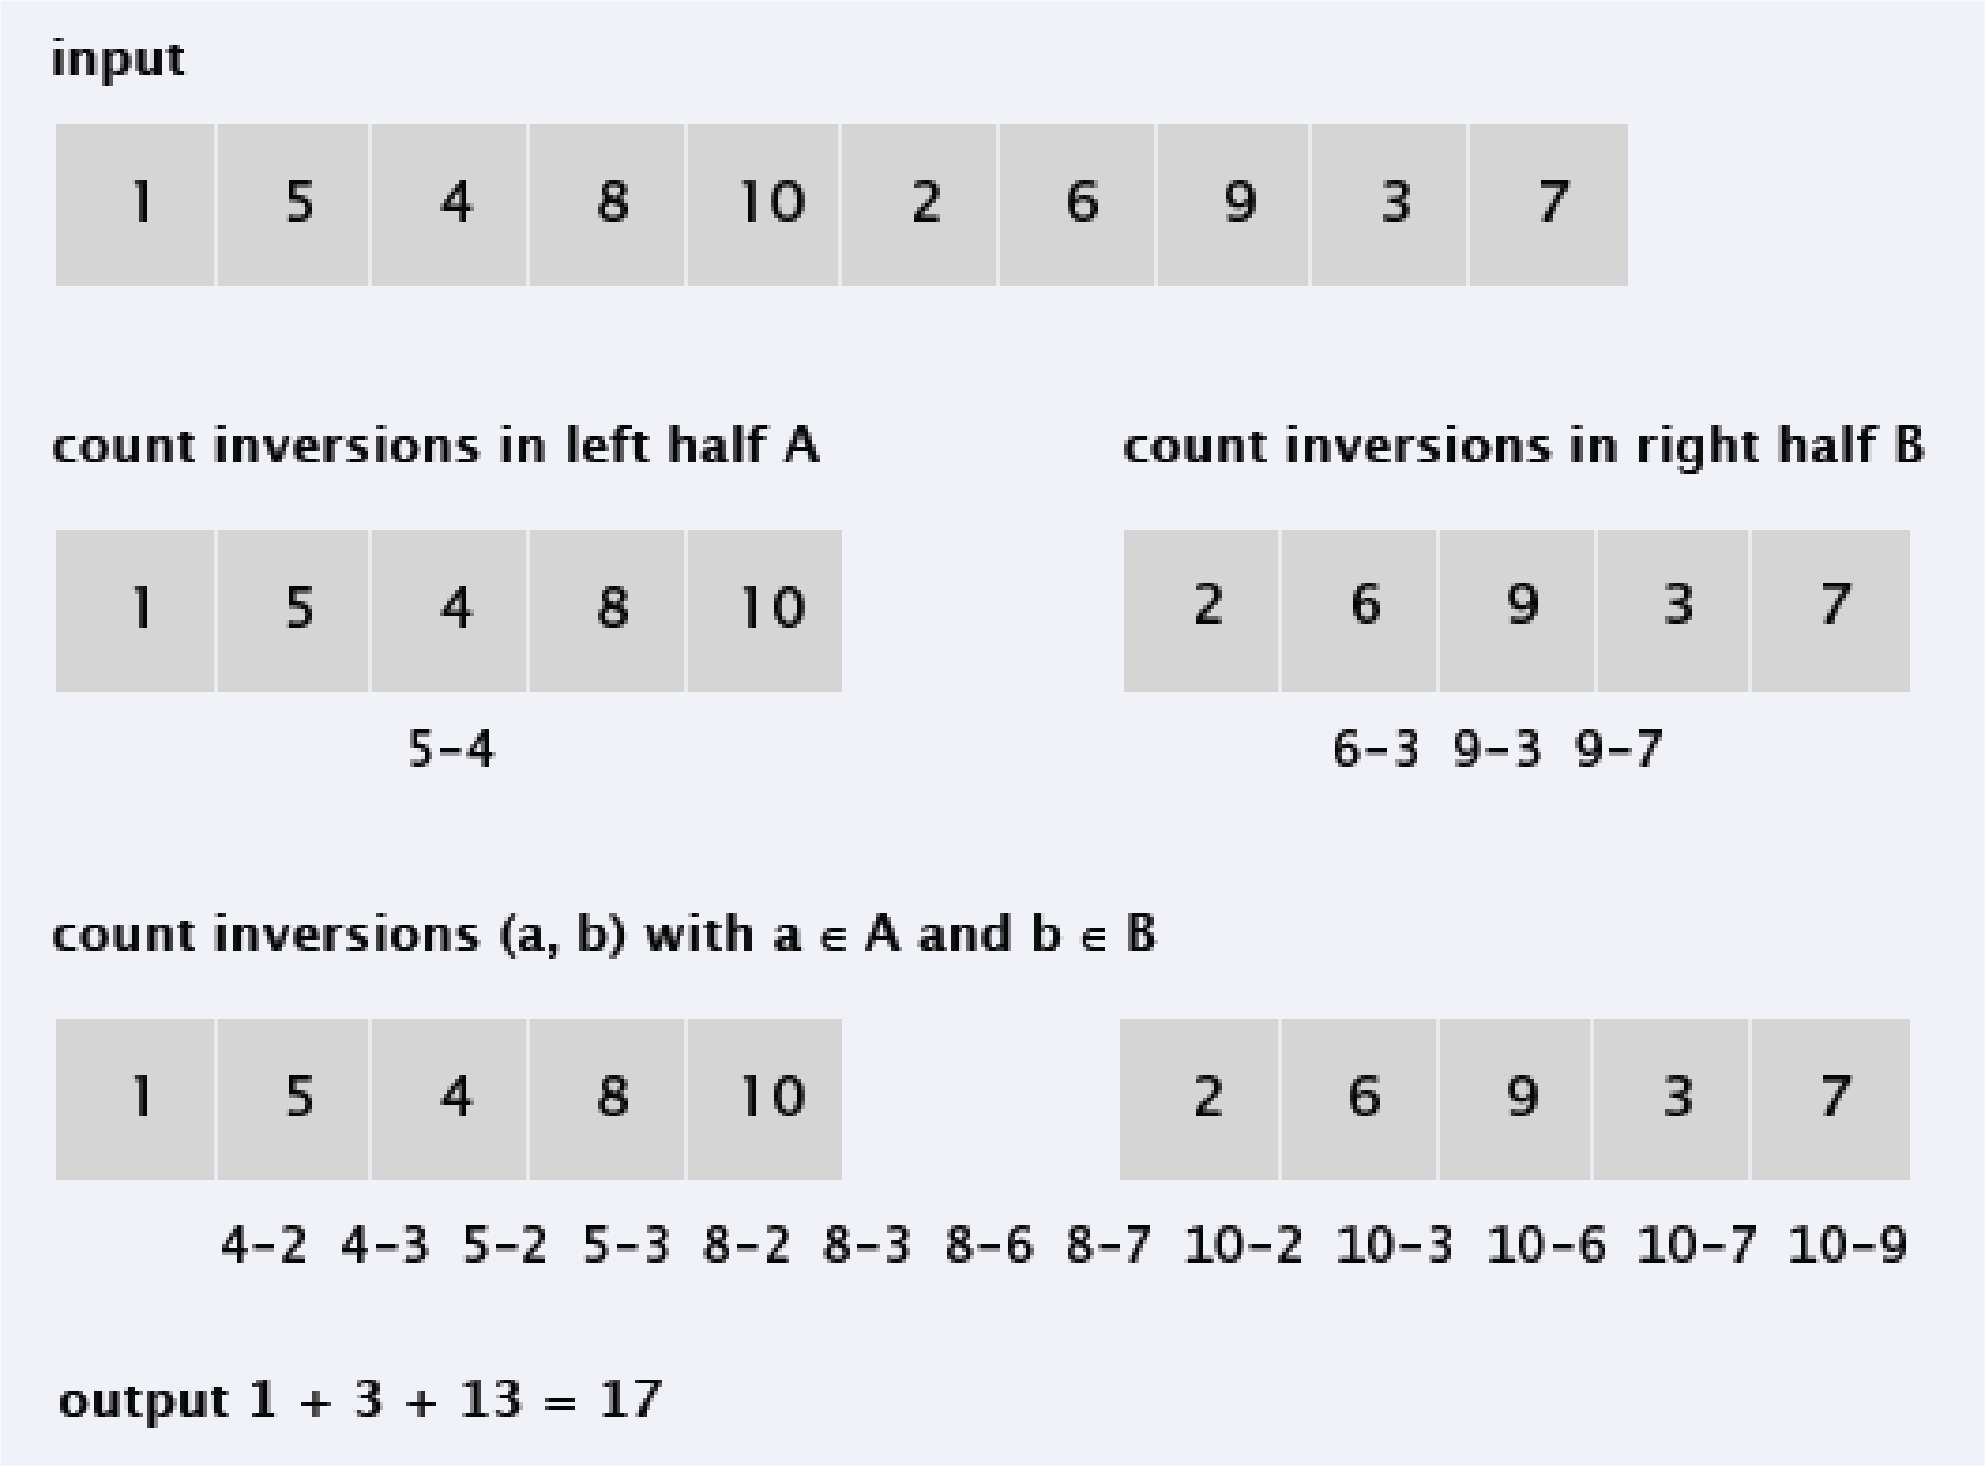
\includegraphics[width=0.5\linewidth]{figures/counting-inversions.png}
\end{center}

Counting inversions $i \in x$ and $j \in y$ is done by merging the two sorted halves.

\begin{itemize}
    \item Scan $x$ and $y$ in parallel from left to right
    \item If $x[i] \le y[j]$, then $x[i]$ is not an inversion
    If $x[i] > y[j]$, then $x[i]$ is an inversion with all elements in $y$ that have not been scanned yet
    \item Append the smaller element to the output array
\end{itemize}

\begin{algorithm}
    \begin{algorithmic}[1]
        \Function{Merge-And-Count}{$L, R$}
            \State $i \gets 1$
            \State $j \gets 1$
            \State $A \gets \emptyset$
            \State $r_{LR} \gets 0$
            \While{$i \le |L|$ and $j \le |R|$}
                \If{$L[i] \le R[j]$}
                    \State $A \gets A \cup \{L[i]\}$
                    \State $i \gets i + 1$
                \Else
                    \State $A \gets A \cup \{R[j]\}$
                    \State $j \gets j + 1$
                    \State $r_{LR} \gets r_{LR} + |L| - i + 1$
                \EndIf
            \EndWhile
            \State \Return $(A \cup L[i \dots] \cup R[j \dots], r_{LR})$
        \EndFunction
    \end{algorithmic}
\end{algorithm}

To formally prove correctness of \textsc{SortAndCount}, we can induce on the size of the array, $n$. 

To analyze the running time of \textsc{SortAndCount}, 

\begin{itemize}
    \item Suppose $T(n)$ is the worst-case running time for inputs of size $n$
    \item Our algorithm satisfies $T(n) \le 2T(\frac{n}{2}) + \mathcal{O}(n)$
    \item Master theorem says this is $T(n) = \mathcal{O}(n \log n)$
\end{itemize}

\section{Master Theorem}

\begin{theorem}[Master Theorem]\index{Master Theorem}
    Let $a \ge 1$ and $b > 1$ be constants, let $f(n)$ be a function, and let $T(n)$ be defined on the nonnegative integers by the recurrence \[
        T(n) \le a \cdot T\left( \frac{n}{b} \right) + f(n)
    \]

    where we interpret $n/b$ to mean either $\lfloor n/b \rfloor$ or $\lceil n/b \rceil$. 
    
    Let $d = \log_b a$. Then, $T(n)$ has the following asymptotic bounds:
    \begin{enumerate}
        \item If $f(n) = \mathcal{O}(n^{d - \epsilon})$ for some constant $\epsilon > 0$, then $T(n) = \mathcal{O}(n^d)$.

        This is the \bred{merge heavy} case. The cost of merging dominates the cost of recursion.

        \item If $f(n) = \mathcal{O}(n^d \log^k n)$, then $T(n) = \mathcal{O}(n^d \log^{k+1} n)$.

        This is the \bred{balanced} case. The cost of merging and recursion are the same.

        \item If $f(n) = \mathcal{O}(n^{d + \epsilon})$ for some constant $\epsilon > 0$, then $T(n) = \mathcal{O}(f(n))$.

        This is the \bred{leaf (recursion) heavy} case. The cost of recursion dominates the cost of merging.
    \end{enumerate}
\end{theorem}

\begin{figure}[ht!]
    \centering

    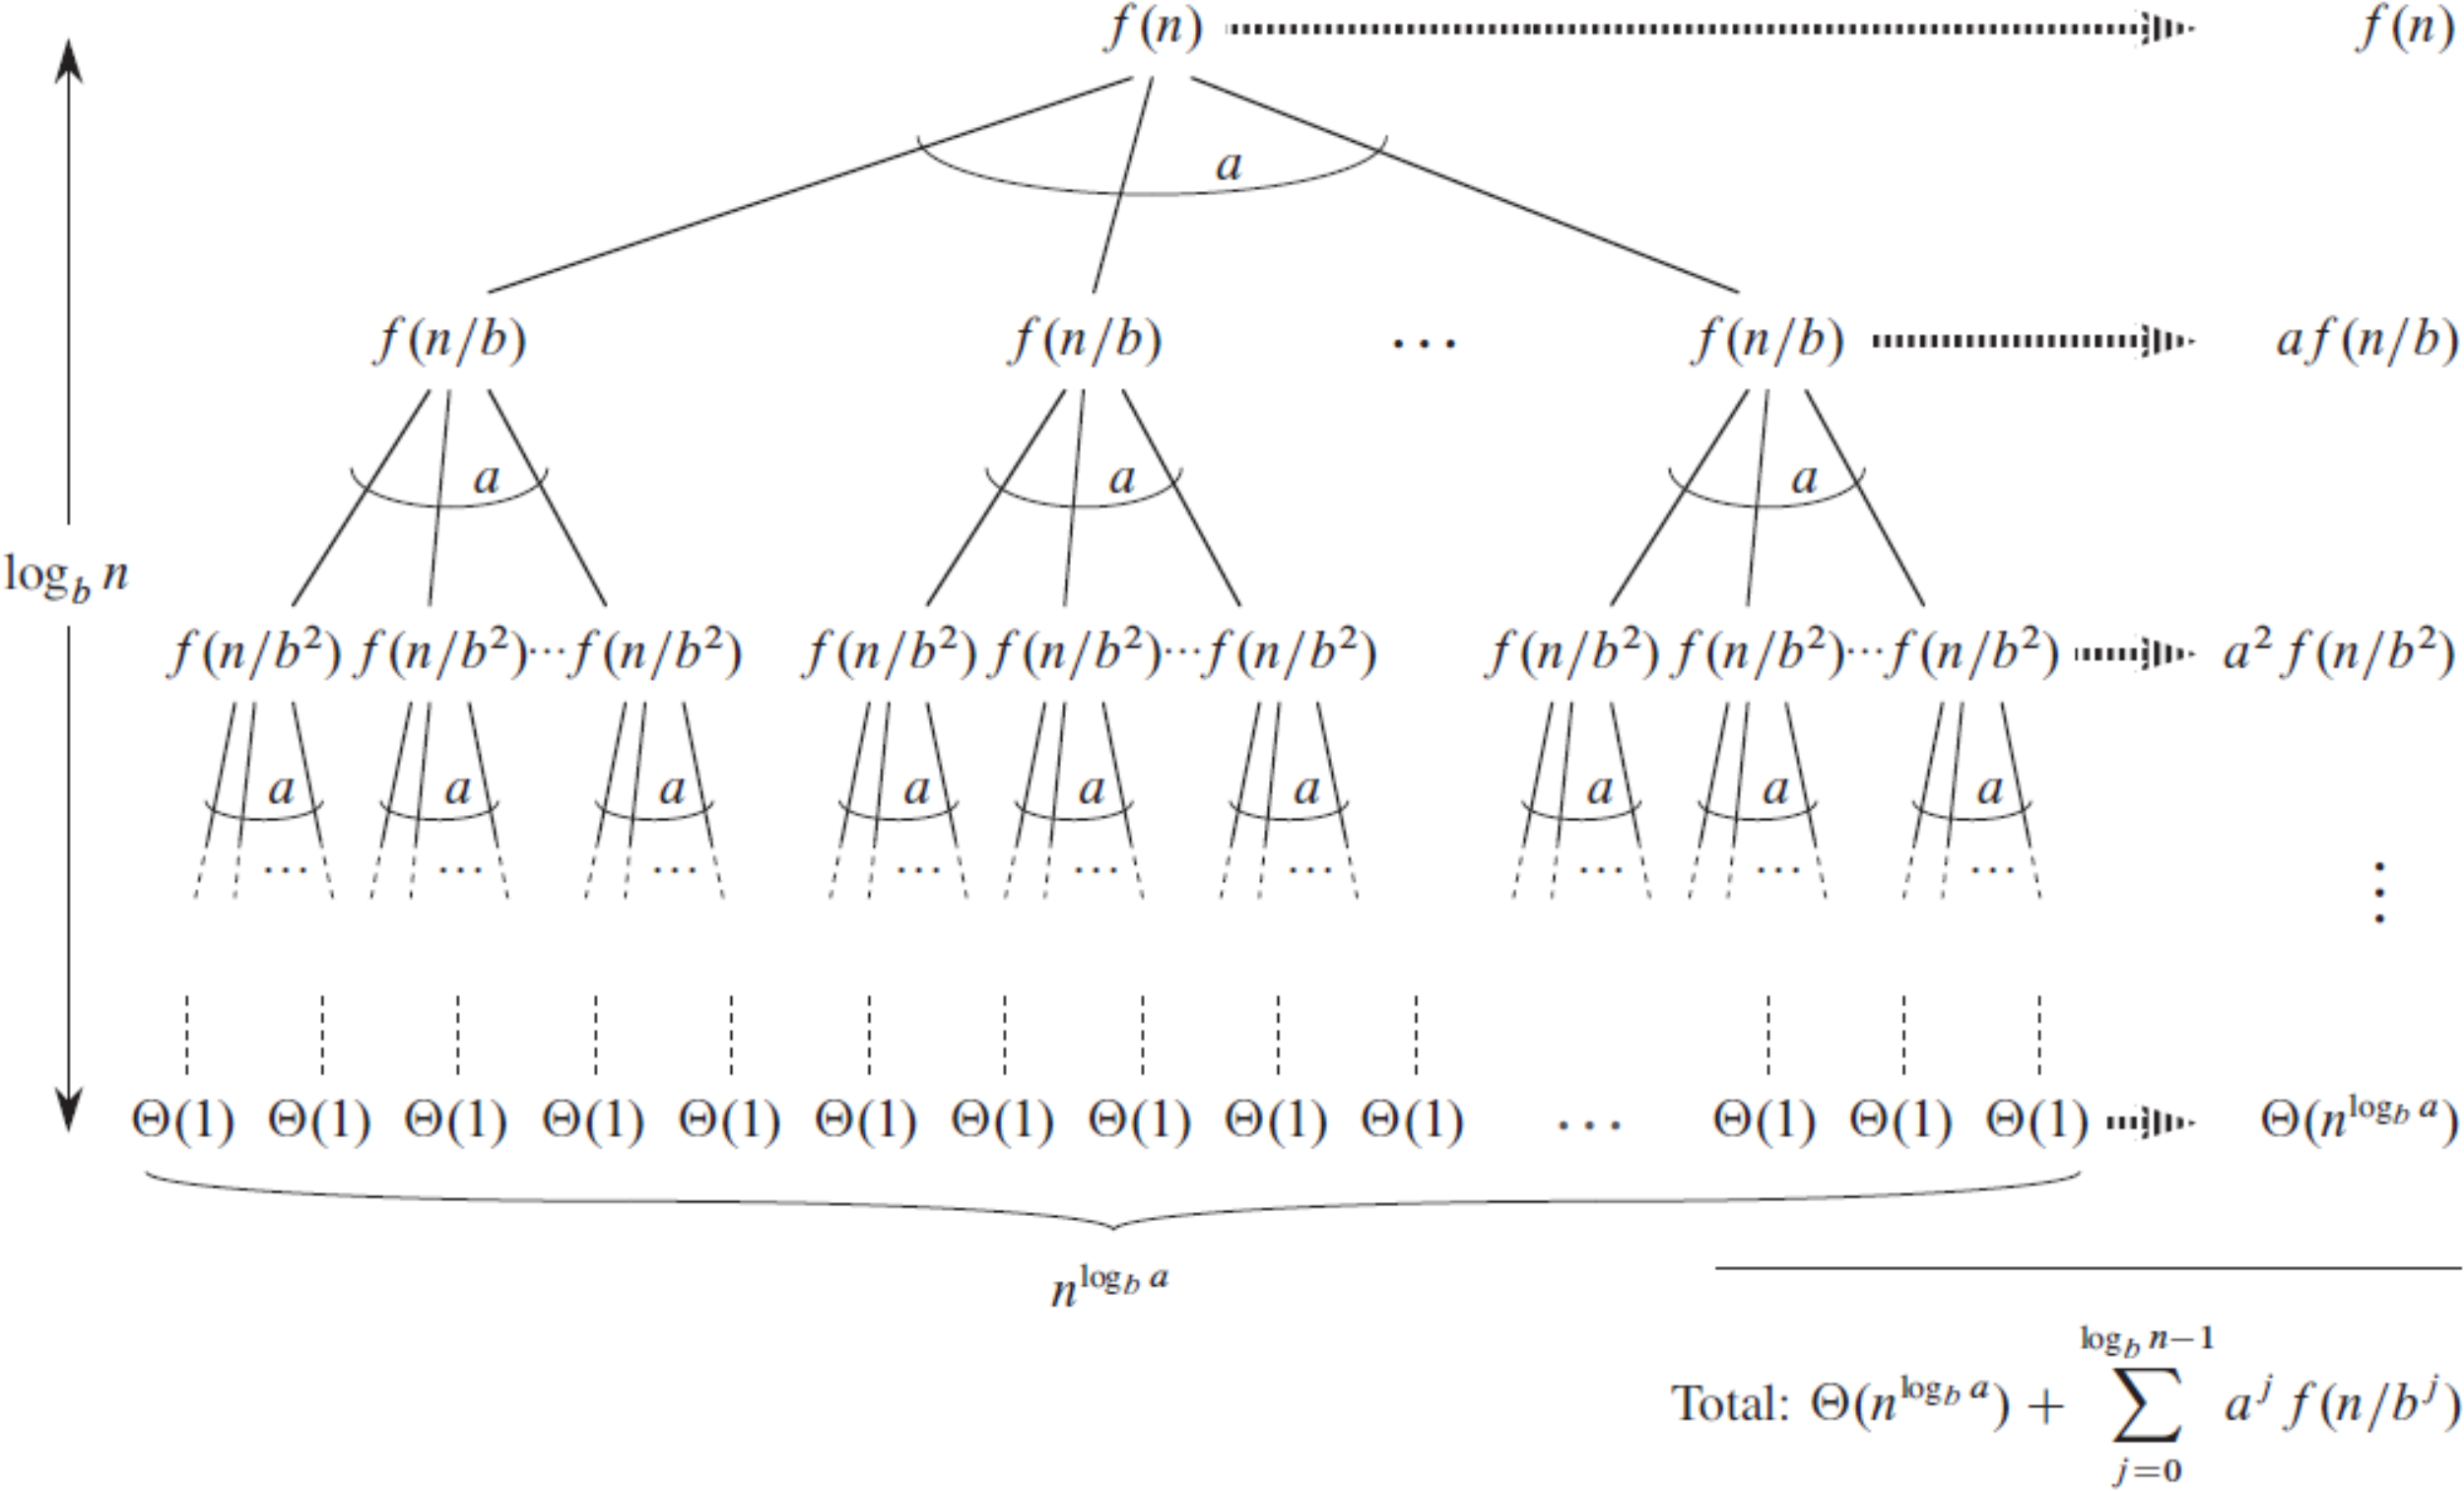
\includegraphics[width=\linewidth]{figures/master-theorem.png}
\end{figure}

\subsection{Closest Pair}

\begin{itemize}
    \item \textbf{Problem}
    
    Given $n$ points of the form $(x_i, y_i)$ in the plane, find the closest pair of points.

    \item \textbf{Applications}
    
    \begin{itemize}
        \item Basic primitive in graphics and computer vision
        \item Geographic information systems, molecular modeling, air traffic control
        \item Special case of nearest neighbor
    \end{itemize}

    \item \textbf{Brute force} is $\mathcal{O}(n^2)$.
\end{itemize}

We can use the divide and conquer paradigm to solve this problem.

\begin{itemize}
    \item \textbf{Divide}: Split the points into two equal halves by drawing a vertical line $L$ through the median $x$-coordinate

    \begin{center} 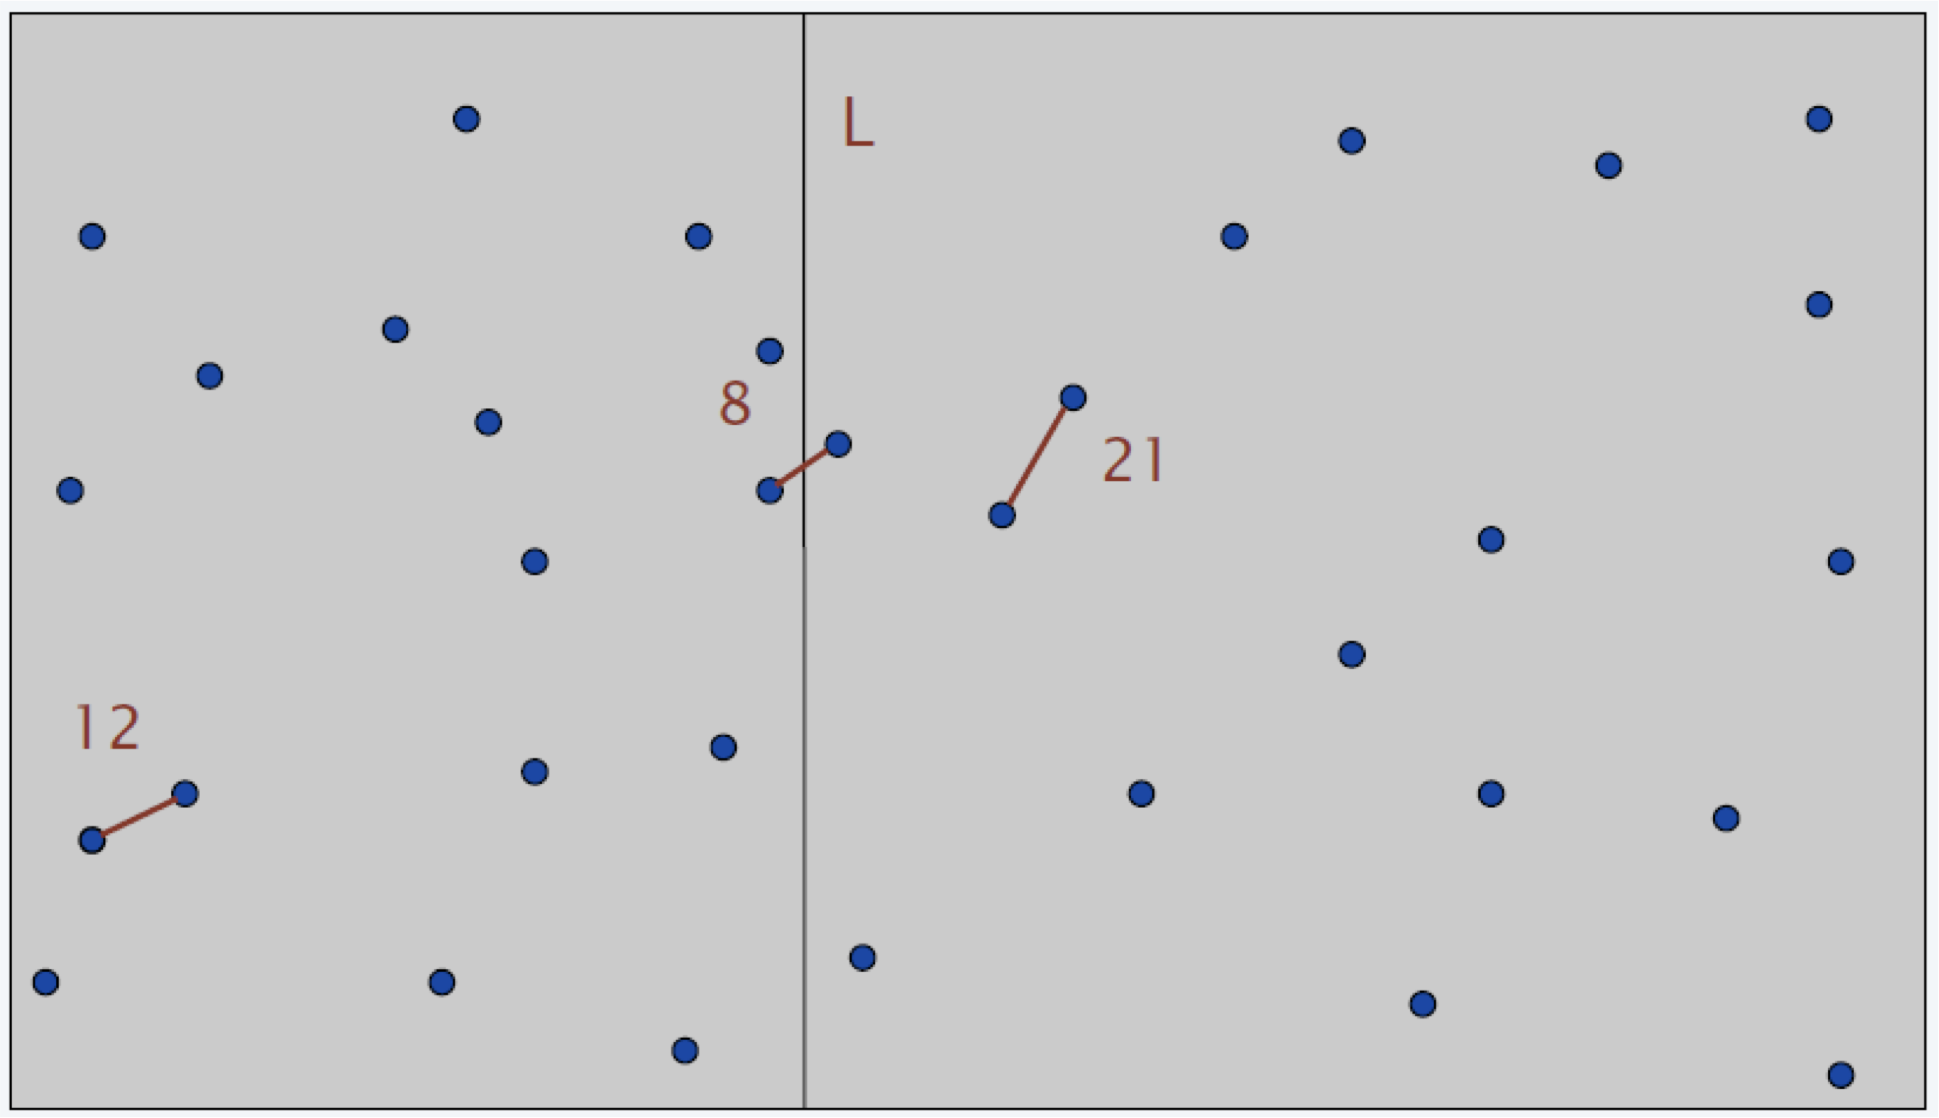
\includegraphics[width=0.55\linewidth]{figures/Closest Pair Divide.png} \end{center}

    \item \textbf{Conquer}: Find the closest pair of points in each half recursively

    \item \textbf{Combine}: Find the closest pair of points with one point in each half

    We can restrict our attention to points within $\delta$ of $L$ on each side, where $\delta = $ best of the solutions within the two halves. 

    \begin{center} 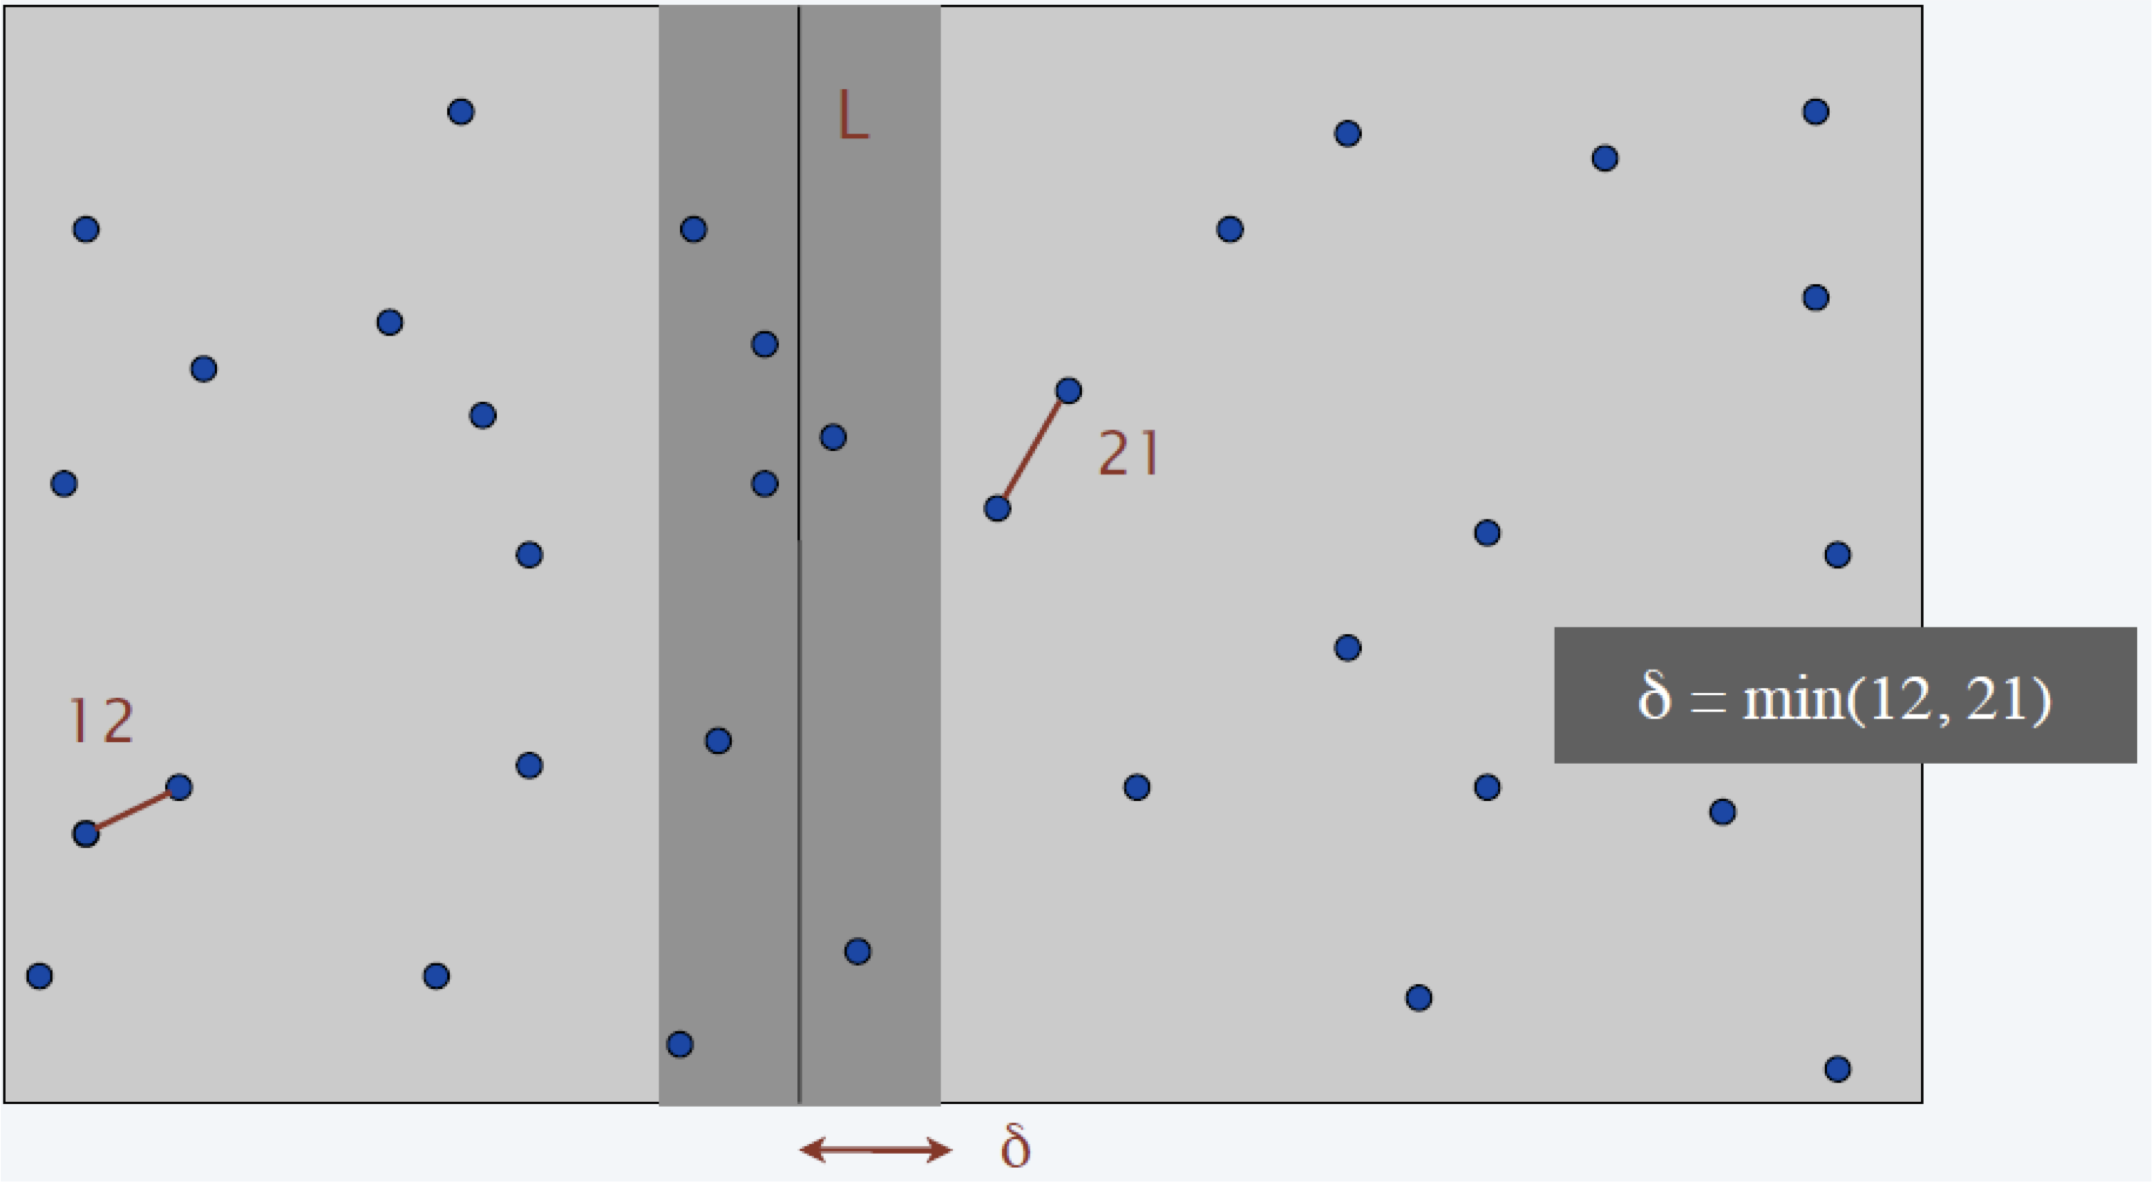
\includegraphics[width=0.55\linewidth]{figures/Closest Pair Conquer.png} \end{center}

    \begin{itemize}
        \item Only need to look at points within $\delta$ of $L$ on each side
        \item Sort points on the strip by $y$ coordinate
        \item Only need to check each point with next 11 points in sorted list
    \end{itemize}

    \item Return the best of 3 solutions
\end{itemize}

\begin{remark}
    \begin{minipage}[t]{0.55\linewidth}
        We chose the number $11$ on purpose.

        \begin{claim}
            If two points are at least $12$ positions apart in the sorted list, their distance is at least $\delta$.
        \end{claim}

        \begin{proof}
            {~~~}

            \begin{itemize}
                \item No two points lie in the same $\frac{\delta}{2} \times \delta$ rectangle.

                \item Two points that are more than two rows apart are at distance $\delta$.
            \end{itemize}
        \end{proof}
    \end{minipage}
    \hfill
    \begin{minipage}[t]{0.4\linewidth}
        \begin{center} \raisebox{-0.9\height}{ 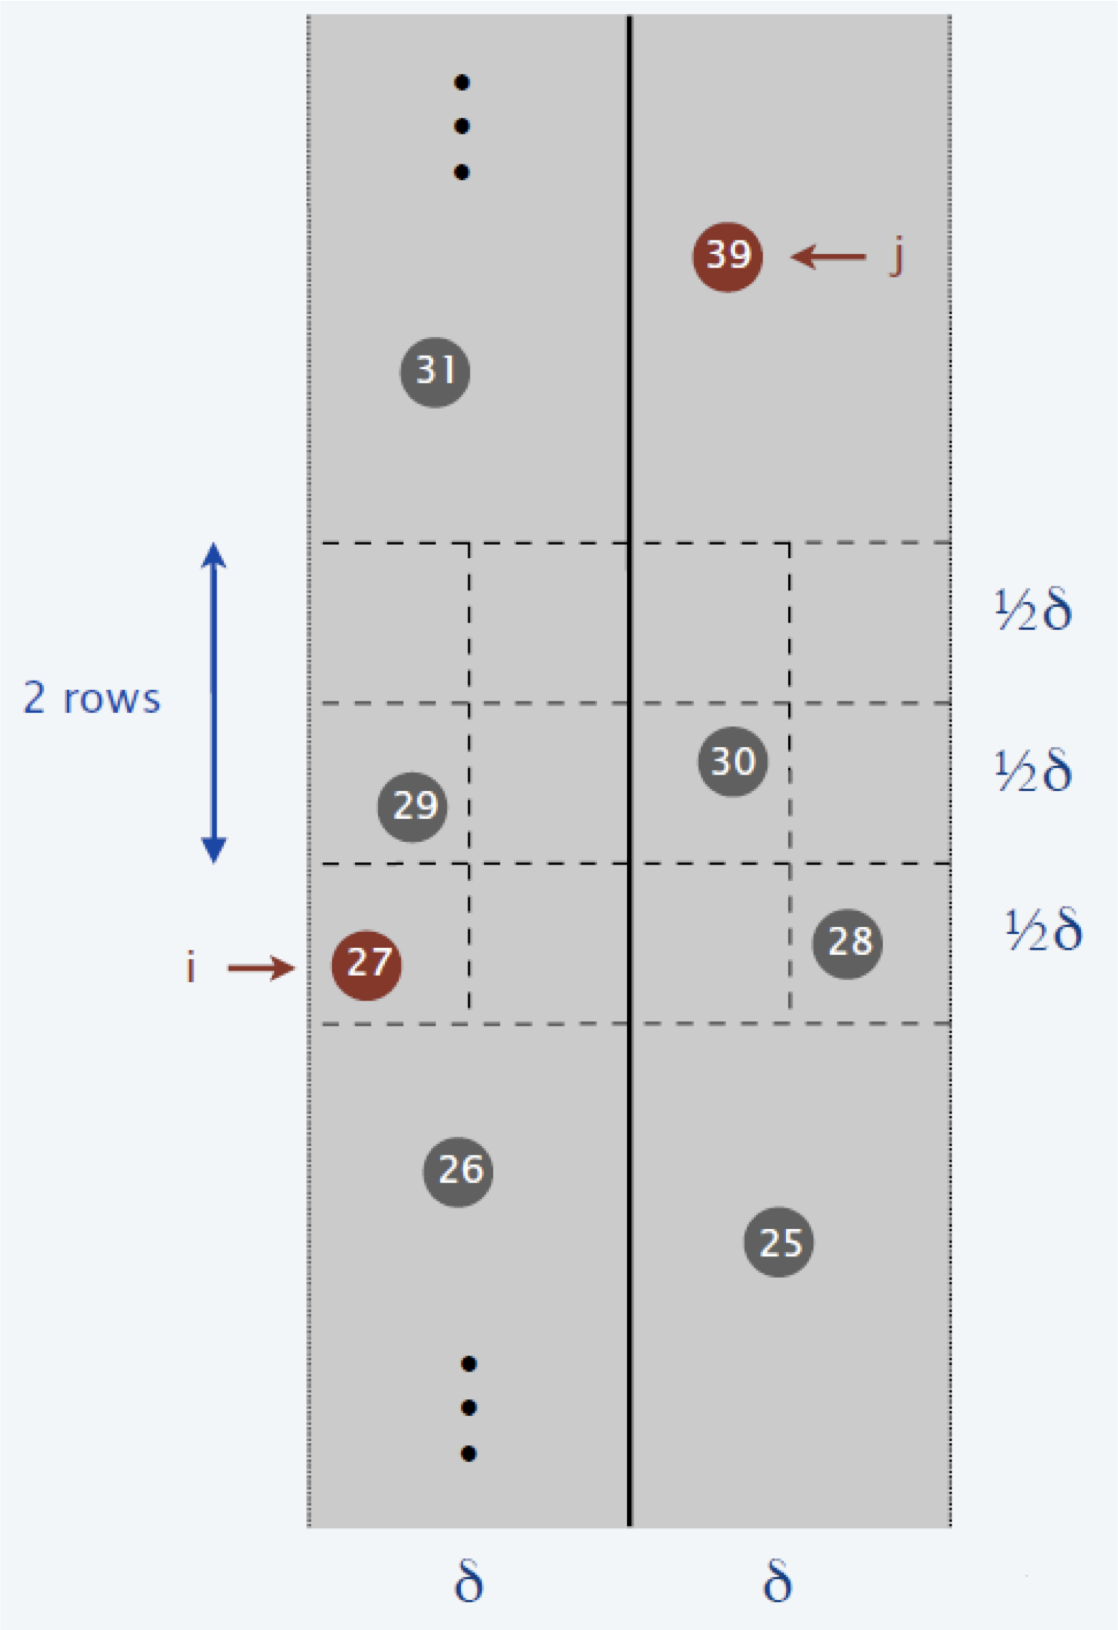
\includegraphics[width=0.9\linewidth]{figures/Closest Pair Grid.png} } \end{center}
    \end{minipage}
\end{remark}

Let $T(n)$ be the worst-case running time of the algorithm. To analyze the Running time for the combine operation, 
\begin{itemize}
    \item Finding points on the strip is $\mathcal{O}(n)$
    \item Sorting points on the strip by their $y$-coordinate is $\mathcal{O}(n \log n)$
    \item Testing each point against 11 points is $\mathcal{O}(n)$
\end{itemize}

Thus, the total running running time is \[
    T(n) \le 2T\left( \frac{n}{2} \right) + \mathcal{O}(n \log n)
\] 

By the master theorem, this yields $T(n) = \mathcal{O}(n \log^2 n)$.

\subsection{Multiplication Algorithms}

\subsubsection{Karatsuba's Algorithm}\index{Karatsuba's Algorithm}\label{subsubsec:karatsuba}

\begin{itemize}
    \item \textbf{Problem}
    
    Given two $n$-bit integers $x$ and $y$, compute their product $xy$.

    \item \textbf{Applications}
    
    \begin{itemize}
        \item Multiplying large integers
        \item Multiplying large polynomials
        \item Multiplying large matrices
    \end{itemize}

    \item \textbf{Brute force} is $\mathcal{O}(n^2)$.
\end{itemize}

Karatsuba's observed that we can divide each integer into two halves, \[
    x = x_1 \cdot 10^{\frac{n}{2}} + x_2  \qquad y = y_1 \cdot 10^{\frac{n}{2}} + y_2
\] and then \[
    xy = (x_1y_1) \cdot 10^n + (x_1y_2 + x_2y_1) \cdot 10^{\frac{n}{2}} + x_2y_2
\] so four $n/2$-bit integer multiplications can be replaced by three: \[
    x_1y_2 + x_2y_1 = (x_1 + x_2)(y_1 + y_2) - x_1y_1 - x_2y_2
\] This would give a running time of \[
    T(n) \le 3T\left( \frac{n}{2} \right) + \mathcal{O}(n) \implies T(n) = \mathcal{O}(n^{\log_2 3}) \approx \mathcal{O}(n^{1.59})
\]

\subsubsection{Strassen's Algorithm}

Strassen's algorithm is a generalization of \hyperref[subsubsec:karatsuba]{Karatsuba's algorithm} to design a fast algorithm for multiplying two $n \times n$ matrices.

\begin{itemize}
    \item We call $n$ the ``size'' of the problem \[
        \begin{bmatrix}
            C_{11} & C_{12} \\
            C_{21} & C_{22}
        \end{bmatrix} = \begin{bmatrix}
            A_{11} & A_{12} \\
            A_{21} & A_{22}
        \end{bmatrix} \begin{bmatrix}
            B_{11} & B_{12} \\
            B_{21} & B_{22}
        \end{bmatrix}
    \]

    \item Nat\"ively, this requires $2^3 = 8$ matrix multiplications of size $\frac{n}{2}$. 
    
    \item Strassen's algorithm reduces this to $7$ matrix multiplications instead of $8$. \[
        T(n) \le 7T\left( \frac{n}{2} \right) + \mathcal{O}(n^2) \implies T(n) = \mathcal{O}(n^{\log_2 7}) \approx \mathcal{O}(n^{2.81})
    \]
\end{itemize}
\vspace{-2em}
\begin{algorithm}
    \begin{algorithmic}[1]
        \Function{Strassen}{$n, A, B$}
        \If{$n = 1$}
            % \State \Return $A \times B$
            \Return $A \times B$
        \EndIf

        {~~~}

        \State Partition $A$ and $B$ into $2 \times 2$ block matrices
        \State $P_1 \gets \Call{Strassen}{\frac{n}{2}, A_{11}, (B_{12} - B_{22})}$
        \State $P_2 \gets \Call{Strassen}{\frac{n}{2}, (A_{11} + A_{12}), B_{22}}$
        \State $P_3 \gets \Call{Strassen}{\frac{n}{2}, (A_{21} + A_{22}), B_{11}}$
        \State $P_4 \gets \Call{Strassen}{\frac{n}{2}, A_{22}, (B_{21} - B_{11})}$
        \State $P_5 \gets \Call{Strassen}{\frac{n}{2}, (A_{11} + A_{22}), (B_{11} + B_{22})}$
        \State $P_6 \gets \Call{Strassen}{\frac{n}{2}, (A_{12} - A_{22}), (B_{21} + B_{22})}$
        \State $P_7 \gets \Call{Strassen}{\frac{n}{2}, (A_{11} - A_{21}), (B_{11} + B_{12})}$

        {~~~}

        \State $C_{11} \gets P_5 + P_4 - P_2 + P_6$
        \State $C_{12} \gets P_1 + P_2$
        \State $C_{21} \gets P_3 + P_4$
        \State $C_{22} \gets P_1 + P_5 - P_3 - P_7$

        {~~~}

        \State \Return $C$
        \EndFunction
    \end{algorithmic}
\end{algorithm}

\subsection{Median and Selection}

\begin{itemize}
    \item \textbf{Selection}
    
    \begin{itemize}
        \item Given an array $A$ of $n$ comparable elements, find the $k$-th smallest element in $A$. 
        \item $k = 1$ is the minimum, $k = n$ is the maximum, and $k = \floor{\frac{n}{2}}$ is the median. 
        \item The running time is $\mathcal{O}(n)$ for minimum and maximum. 
    \end{itemize}

    \item \textbf{$k$-Selection}

    \begin{itemize}
        \item $\bigo{nk}$ by modifying bubble sort.
        \item $\bigo{n \log n}$ by sorting. 
        \item $\bigo{n + k \log n}$ by using a min-heap.
        \item $\bigo{k + n \log k}$ by using a max-heap.
        \item $\bigo{n}$ by using the divide and conquer paradigm.
    \end{itemize}
\end{itemize}

\subsubsection{QuickSelect}

\begin{itemize}
    \item \textbf{Divide}: Pick a pivot $p$ at random from $A$

    \item \textbf{Conquer}: Partition $A$ into two sub-arrays 
    
    \begin{itemize}
        \item $A_{less}$ contains all elements less than $p$
        \item $A_{more}$ contains all elements greater than $p$
    \end{itemize}

    \item \textbf{Combine}: 
    \begin{itemize}
        \item If $|A_{less}| \ge k$, return $k$-th smallest element in $A_{less}$
        \item Otherwise, return $(k - |A_{less}|)$-th smallest element in $A_{more}$
    \end{itemize}
\end{itemize}

However, this algorithm is not guaranteed to be $\mathcal{O}(n)$, as the pivot may be the largest or smallest element in the array. If pivot is close to the min or the max, then we basically get $T(n) \le T(n - 1) + \bigo{n}$, which is $\bigo{n^2}$. We want to reduce $n - 1$ to a fraction of $n$. 

% TODO
\chapter{Greedy Algorithms}

\section{Introduction}

\term{Greedy algorithms} are a class of algorithms that make locally optimal choices at each step in order to find a global optimum. They are often used to solve optimization problems.

\begin{listu}
    \item \textbf{Goal:} find a solution $x$ maximizing or minimizing some objective function $f$.
    \item \textbf{Challenge:} space of possible solutions $x$ is too large to search exhaustively.
    \item \textbf{Insight:} $x$ is composed of several parts (e.g., $x$ is a set or a sequence).
    \item \textbf{Approach:} instead of computing $x$ directly,
    \begin{listu}
        \item Compute $x$ one part at a time.
        \item Select the next part ``greedily'' to get the most immediate ``benefit'', which needs to be defined carefully for each problem.
        \item Polynomial running time is typically guaranteed.
        \item Need to prove that this will always return an optimal solution despite having no global view of the problem.
    \end{listu}
\end{listu}

\section{Interval Scheduling}

\subsection{Problem Definition}

\begin{listu}
    \item Job $j$ starts at time $s_j$ and finishes at time $f_j$.
    \item Two jobs $i$ and $j$ are compatible if $[s_i, f_i)$ and $[s_j, f_j)$ do not overlap.
    \item \textbf{Goal:} find a maximum-size subset of mutually compatible jobs.
\end{listu}

\subsection{Greedy Algorithm}

The greedy algorithm for interval scheduling follows the template
\begin{listu}
    \item Consider jobs in some ``natural'' order.
    \item Take a job if it is compatible with the ones already taken.
\end{listu}

But, what is the ``natural'' order?
\begin{listu}
    \item \textbf{Earliest start time:} ascending order of $s_j$.
    \item \textbf{Earliest finish time:} ascending order of $f_j$.
    \item \textbf{Shortest interval:} ascending order of $f_j - s_j$.
    \item \textbf{Fewest conflicts:} ascending order of $c_j$, where $c_j$ is the number of remaining jobs that conflicts with job $j$.
\end{listu}

However, not all of these orders will yield the optimal solution. Below are some counterexamples.

{~~~}

\begin{minipage}[t]{0.55\linewidth}
    \begin{center} \tikzexternalenable 
\begin{tikzpicture}[baseline=(current bounding box.center)]
        \definecolor{lightGray}{gray}{0.7}
        \definecolor{darkGray}{gray}{0.5}

        \node[draw=none, fill=lightGray, minimum width=1cm, minimum height=0.25cm] at (0, 0) {};
        \node[draw=none, fill=lightGray, minimum width=1cm, minimum height=0.25cm] at (1.5, 0) {};
        \node[draw=none, fill=lightGray, minimum width=1cm, minimum height=0.25cm] at (3, 0) {};
        \node[draw=none, fill=lightGray, minimum width=1cm, minimum height=0.25cm] at (4.5, 0) {};

        \node[draw=none, fill=darkGray, minimum width=6.5cm, minimum height=0.25cm] at (2.25, -0.375) {};
    \end{tikzpicture} \tikzexternaldisable \end{center}
\end{minipage}
\begin{minipage}[t]{0.35\linewidth}
    \begin{center}
        Earliest Start Time
    \end{center}
\end{minipage}

{~~~}

{~~~}

\begin{minipage}[t]{0.55\linewidth}
    \begin{center} \tikzexternalenable 
\begin{tikzpicture}[baseline=(current bounding box.center)]
        \definecolor{lightGray}{gray}{0.7}
        \definecolor{darkGray}{gray}{0.5}

        \node[draw=none, fill=lightGray, minimum width=2cm, minimum height=0.25cm] at (0, 0) {};
        \node[draw=none, fill=lightGray, minimum width=2cm, minimum height=0.25cm] at (2.5, 0) {};

        \node[draw=none, fill=darkGray, minimum width=1.5cm, minimum height=0.25cm] at (1.25, -0.375) {};
    \end{tikzpicture} \tikzexternaldisable \end{center}
\end{minipage}
\begin{minipage}[t]{0.35\linewidth}
    \begin{center}
        Shortest Interval
    \end{center}
\end{minipage}

{~~~}

{~~~}

\begin{minipage}[t]{0.55\linewidth}
    \begin{center} \tikzexternalenable 
\begin{tikzpicture}[baseline=(current bounding box.center)]
        \definecolor{lightGray}{gray}{0.7}
        \definecolor{darkGray}{gray}{0.5}

        \node[draw=none, fill=lightGray, minimum width=1cm, minimum height=0.25cm] at (0, 0) {};
        \node[draw=none, fill=lightGray, minimum width=1cm, minimum height=0.25cm] at (1.5, 0) {};
        \node[draw=none, fill=lightGray, minimum width=1cm, minimum height=0.25cm] at (3, 0) {};
        \node[draw=none, fill=lightGray, minimum width=1cm, minimum height=0.25cm] at (4.5, 0) {};

        \node[draw=none, fill=lightGray, minimum width=1cm, minimum height=0.25cm] at (0.75, -0.375) {};
        \node[draw=none, fill=lightGray, minimum width=1cm, minimum height=0.25cm] at (0.75, -0.75) {};
        \node[draw=none, fill=lightGray, minimum width=1cm, minimum height=0.25cm] at (0.75, -1.125) {};

        \node[draw=none, fill=lightGray, minimum width=1cm, minimum height=0.25cm] at (3.75, -0.375) {};
        \node[draw=none, fill=lightGray, minimum width=1cm, minimum height=0.25cm] at (3.75, -0.75) {};
        \node[draw=none, fill=lightGray, minimum width=1cm, minimum height=0.25cm] at (3.75, -1.125) {};

        \node[draw=none, fill=darkGray, minimum width=1cm, minimum height=0.25cm] at (2.25, -0.375) {};
    \end{tikzpicture} \tikzexternaldisable \end{center}
\end{minipage}
\begin{minipage}[t]{0.35\linewidth}
    \begin{center}
        Fewest Conflicts
    \end{center}
\end{minipage}

{~~~}

We can implement the greedy algorithm using \bred{earliest finish time order} (EFT).

\begin{listu}
    \item Sort jobs by finish time, say $f_1 \le f_2 \le \dots \le f_n$. \[
        \mathcal{O}(n \log n)
    \]

    \item For each job $j$, we need to check if it's compatible will \itblue{all} previously added jobs.

    \begin{listu}
        \item Natively, this is $\mathcal{O}(n^2)$, as we need $\mathcal{O}(n)$ for each job.
        \item We only need to check if $s_j \ge f_{i^*}$, where $i^*$ is the \itblue{last job added}.
        \begin{listu}
            \item For any jobs $i$ added before $i^*$, we have $f_i \le f_{i^*}$.
            \item By keeping track of $f_{i^*}$, we can check compatibility of job $j$ in $\mathcal{O}(1)$.
        \end{listu}
    \end{listu}

    \item Thus, the total running time is \[
        \mathcal{O}(n \log n).
    \]
\end{listu}

\subsection{Proof of Optimality}

\subsubsection{By Contradiction}

\begin{listu}
    \item Suppose for contradiction that greedy is not optimal

    \item Say greedy selects jobs $i_1, i_2, \dots, i_k$ sorted by finish time

    \item Consider an optimal solution $j_1, j_2, \dots, j_m$ sorted by finish time which matches greedy for as many indices as possible.

    That is, $j_1 = i_1, j_2 = i_2, \dots, j_r = i_r$ for the greatest possible $r$.

    \item Both $i_{r+1}$ and $j_{r+1}$ must be compatible with the previous selection $i_1, i_2, \dots, i_r = j_1, j_2, \dots, j_r$.

    \item Consider a new solution $i_1, i_2, \dots, i_r, {\color{red}j_{r+1}}, {\color{lightBlue}j_{r+2}, \dots, j_m}$.

    \begin{listu}
        \item We have replaced $j_{r+1}$ by $i_{r+1}$ in our reference optimal solution
        \item This is still \bred{feasible} because $f_{i_{r+1}} \le f_{j_{r+1}} \le s_{j_{t}}$ for $t \ge r+2$.
        \item This is still \bred{optimal} because $m$ jobs are sorted.
        \item But it matched the greedy solution in $r + 1$ indices. This is a contradiction.
    \end{listu}
\end{listu}

\begin{center}
    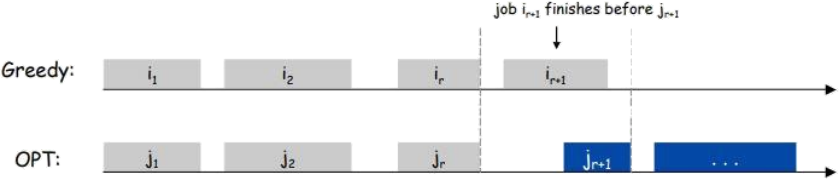
\includegraphics[width=0.67\linewidth]{figures/interval-scheduling-contradiction.png}
\end{center}

\subsubsection{By Induction}

\begin{listu}
    \item Let $S_j$ be the subset of jobs picked by greedy after considering the first $j$ jobs in the increasing order of finish time.

    Define $S_0 = \varnothing$.

    \item We call this partial solution \bred{promising} if there is a way to extend it to an optimal solution by picking some subset of jobs $j + 1, \dots, n$.

    $\exists T \subseteq \{j + 1, \dots, n\}$ such that $S_j \cup T$ is an optimal solution.

    \item \bred{Inductive claim:} for all $t \in \{0, 1, \dots, n\}$, $S_t$ is promising.

    \begin{listu}
        \item For $t = n$, if $S_n$ is promising, then it must be an optimal solution.

        \item We choose $t = 0$ as our base case since it is trivially promising.
    \end{listu}

    \item \textbf{Base case:} $t = 0$.

    For $t = 0$, $S_0 = \varnothing$ is promising. Any optimal solution extends it.

    \item \textbf{Inductive step:} $t - 1 \to t$.

    Suppose the claim holds for $t = j - 1$ and optimal solution $O_{j-1}$ extends $S_{j-1}$.

    At $t = j$, we have two cases:

    \begin{listo}
        \item Greedy did not select job $j$, so $S_j = S_{j-1}$.

        \begin{listu}
            \item Job $j$ must conflict with some job in $S_{j-1}$.
            \item Since $S_{j-1} \subseteq O_{j-1}$, $O_{j-1}$ also include pick job $j$.
            \item $O_j = O_{j-1}$ also extends $S_j = S_{j-1}$.
        \end{listu}

        \item Greedy selected job $j$, so $S_j = S_{j-1} \cup \{j\}$.

        \begin{listu}
            \item Consider the earliest job $r$ in $O_{j-1} \setminus S_{j-1}$.
            \item Consider $O_j$ contained by replacing $r$ with $j$ in $O_{j-1}$.
            \item Prove that $O_j$ is still feasible.
            \item $O_j$ extends $S_j$, as desired.
        \end{listu}

        \begin{center}
            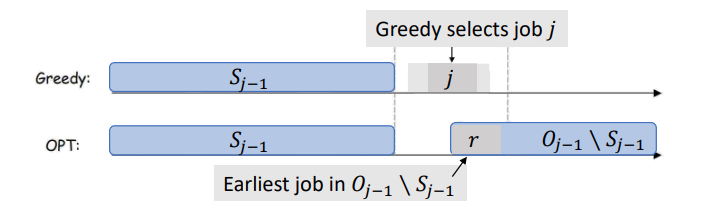
\includegraphics[width=0.67\linewidth]{figures/interval-scheduling-induction.png}
        \end{center}
    \end{listo}
\end{listu}

\subsubsection{Contradiction vs Induction}

Both methods make the same claim, that \begin{center}
    ``The greedy solution after $j$ iterations can be extended to an optimal solution, $\forall j$''.
\end{center} They also use the same key argument. \begin{center} \begin{minipage}[t]{0.9\linewidth}
    ``If the greedy solution after $j$ iterations can be extended to an optimal solution, then the greedy solution after $j + 1$ iterations can be extended to an optimal solution as well''
\end{minipage}
\end{center}

\begin{listu}
    \item For proof by induction, this is the key induction step.
    \item For proof by contradiction, we take the greatest $j$ for which the greedy solution can be extended to an optimal solution, and derive a contradiction by extending the greedy solution after $j + 1$ iterations.
\end{listu}

\section{Interval Partitioning}

\subsection{Problem Definition}

\begin{listu}
    \item Job $j$ starts at time $s_j$ and finishes at time $f_j$.
    \item Two jobs are compatible if they do not overlap.
    \item \textbf{Goal:} group jobs into fewest partitions such that jobs in the same partition are compatible.
\end{listu}

\begin{example}
    Think of scheduling lectures for various courses into as few classrooms as possible.

    This schedule uses \bred{4} classrooms for scheduling 10 lectures, but we can do better.

    \begin{center}
        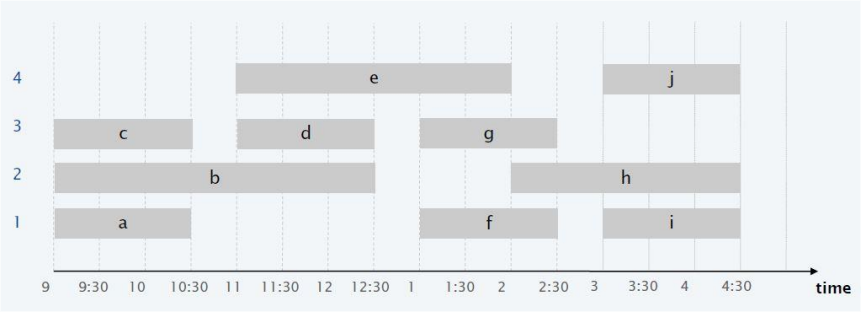
\includegraphics[width=0.55\linewidth]{figures/interval-scheduling-4-classrooms.png}
    \end{center}

    This schedule uses \bred{3} classrooms for scheduling 10 lectures, which is optimal.

    \begin{center}
        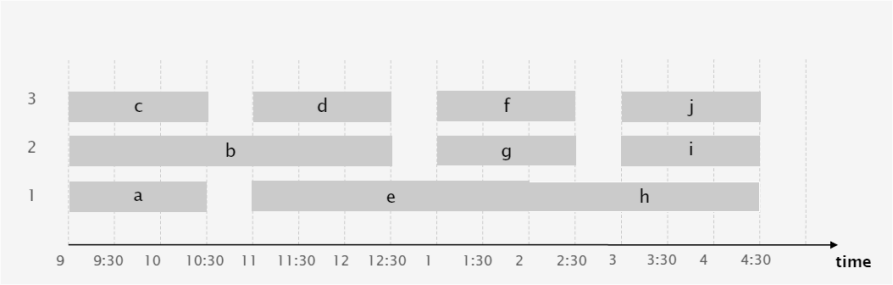
\includegraphics[width=0.55\linewidth]{figures/interval-scheduling-3-classrooms.png}
    \end{center}
\end{example}

One idea to solve this problem is to find the maximum compatible set using the previously greedy EFT algorithm, and then remove these jobs from the set and repeat. However, this is not optimal.

\subsection{Greedy Algorithm}

The greedy algorithm for interval partitioning follows the template

\begin{listu}
    \item Go through lectures in some ``natural'' order.
    \item Assign each lecture to an \itblue{arbitrary} compatible classroom, and create a new classroom if the lecture conflicts with every existing classroom
\end{listu}

If later we figures that arbitrary assignment is not optimal, we may need to go back to this template, and use a more careful assignment strategy.

\begin{minipage}[t]{0.6\linewidth}
    {~~~}

    It still makes sense to use the same ``natural'' orders as before: earliest start time, earliest finish time, shortest interval, and fewest conflicts.

    {~~~}

    Similar to interval scheduling, when we assign each lecture to an arbitrary compatible classroom, three of these heuristics do not work.
\end{minipage}
\hfil%
\begin{minipage}[t]{0.35\linewidth}
    \begin{center}
        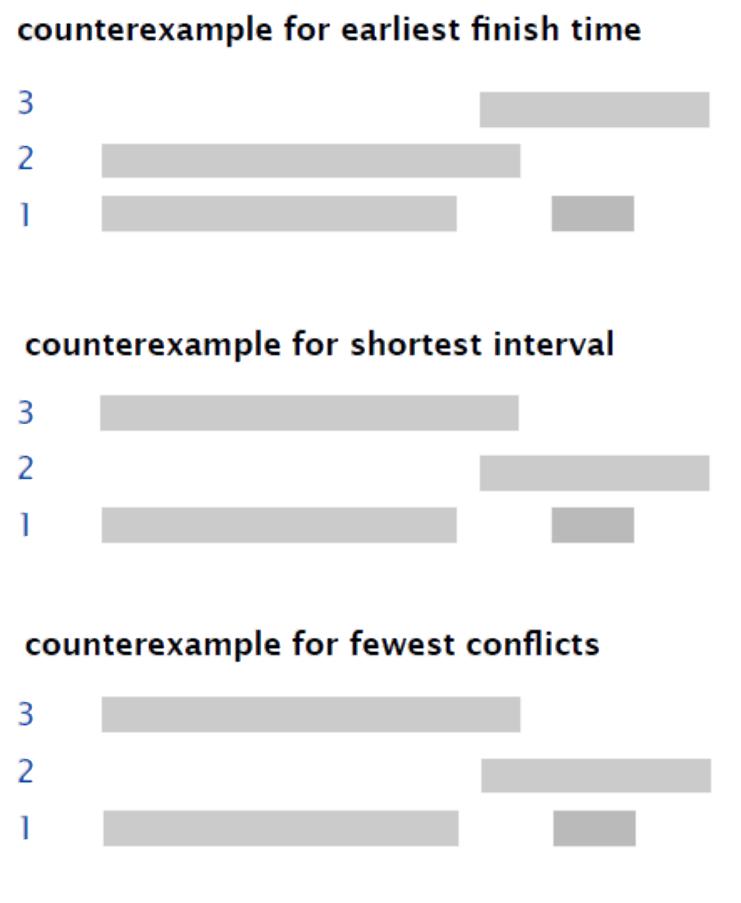
\includegraphics[width=0.9\linewidth,valign=t]{figures/interval-scheduling-counterexample.png}
    \end{center}
\end{minipage}

\begin{algorithm}
    \begin{algorithmic}
        \Function{Earliest-Start-Time-First}{$n, s_1, s_2, \dots, s_n, f_1, f_2, \dots, f_n$}
            \State \Call{Sort}{lectures} bt start time so that $s_1 \le s_2 \le \cdots \le s_n$
            \State $d \gets 0$
            \For{$i = 1$ \To $n$}
                \If{lecture $j$ is compatible with some classroom}
                    \State Schedule lecture $j$ in any such classroom $k$
                \Else
                    \State Allocate a new classroom $d + 1$
                    \State Schedule lecture $j$ in classroom $d + 1$
                    \State $d \gets d + 1$
                \EndIf
            \EndFor

            \State \Return schedule
        \EndFunction
    \end{algorithmic}
\end{algorithm}

\subsubsection{Running Time}

\begin{listu}
    \item \textbf{Key step:} checking if the next lecture can be scheduled at some classroom.

    \item We can tore classrooms in a priority queue, with the key being the latest finish time of any lecture in the classroom.

    \item Determining if lecture $j$ is compatible with some classrooms is equivalent to determining whether $s_j \ge f_k$ for some classroom $k$.

    \begin{listu}
        \item If it is compatible, we add jecture $j$ to classroom $k$ with minimum key, and increase its key to $f_j$.
        \item If it is not compatible, we add a new classroom to the priority queue with key $f_j$.
    \end{listu}

    \item There are $\mathcal{O}(n)$ priority queue operations, each of which takes $\mathcal{O}(\log n)$ time.

    This gives a total running time of \[
        \mathcal{O}(n \log n).
    \]
\end{listu}

\subsection{Proof of Optimality}

\subsubsection{Lower Bound}

The number of classrooms used by any algorithm is at least the number of lectures running at any time, which we call the ``depth''. This is because each classroom can only hold one lecture at a time.

We claim that the greedy algorithm uses only these many classrooms.

\begin{center}
    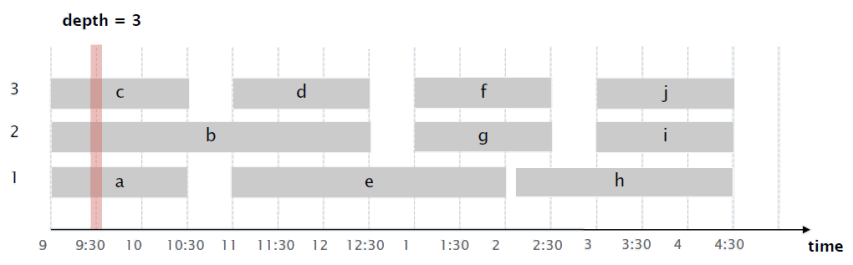
\includegraphics[width=0.75\linewidth]{figures/interval-scheduling-lower-bound.png}
\end{center}

\subsubsection{Upper Bound}

\begin{listu}
    \item Let $d$ be the number of classrooms used by the greedy algorithm.

    \item Classroom $d$ was opened because there was a lecture $j$ which was incompatible with some lectures already scheduled in each of $d - 1$ other classrooms.

    \item All these $d$ lectures end after $s_j$.

    Since we \itblue{have sorted the lectures by start time}, they all start at/before $s_j$.

    \item So, at time $s_j$, we have $d$ mutually overlapping lectures.

    \item Hence, $\text{depth} \ge d$, which is the number of classrooms used by the greedy algorithm.
\end{listu}

By the lower bound and the upper bound, we have that the greedy algorithm is optimal. \qed

\subsection{Interval Graphs}

\begin{definition}
    An \term{interval graph} is a graph whose vertices can be mapped to intervals on the real line such that two vertices are adjacent if and only if their corresponding intervals overlap.
\end{definition}

With this definition, we can restate the interval scheduling and partitioning problems as graph problems.
\begin{listu}
    \item Interval Scheduling: find a maximum independent set (MIS) in an interval graph.
    \item Interval Partitioning: find a minimum coloring of an interval graph.
\end{listu}

MIS and graph coloring are NP-hard for general graphs, but they are efficiently solvable for interval graphs.
\begin{listu}
    \item Graphs which can be obtained from incompatibility of intervals
    \item In fact, this holds even when we are not given an interval representation of the graph
\end{listu}

\section{Minimizing Lateness}

\subsection{Problem Definition}

\begin{listu}
    \item We have a single machine.
    \item Each job $j$ requires $t_j$ units of time and is due by time $d_j$.
    \item If it is scheduled to start at time $s_j$, then it finishes at time $f_j = s_j + t_j$.
    \item The \term{lateness} of job $j$ is defined as $\ell_j = \max\{0, f_j - d_j\}$.
    \item \textbf{Goal:} schedule jobs to minimize the maximum lateness, $L = \max_j \ell_j$.
\end{listu}

To contrast with interval scheduling problems, we now can decide the start time of each job, and the deadlines are soft.

\begin{example}
    Below are some jobs given to us.

    \begin{table}[ht!]
        \centering
        \begin{tabular}{c|c|c|c|c|c|c}
                  & 1 & 2 & 3 & 4 & 5  & 6  \\ \hline
            $t_j$ & 3 & 2 & 1 & 4 & 3  & 2  \\ \hline
            $d_j$ & 6 & 8 & 9 & 9 & 14 & 15 \\
        \end{tabular}
    \end{table}

    An example schedule would be
    \begin{center}
        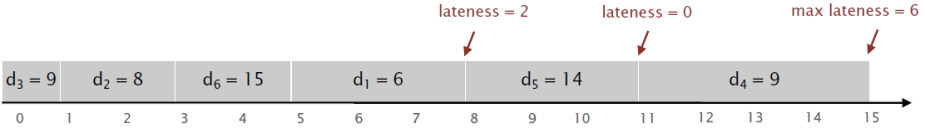
\includegraphics[width=0.8\linewidth]{figures/minimizing-lateness-example.png}
    \end{center}

    Note that this schedule is not optimal.
\end{example}

\subsection{Greedy Algorithm}

The greedy algorithm for minimizing lateness follows the template
\begin{listu}
    \item Consider jobs one-by-one in some ``natural'' order.
    \item Schedule jobs in this order (nothing special to do here, since we have to schedule all jobs and there is only one machine available)
\end{listu}

Here, the ``natural'' order may be
\begin{listu}
    \item \textbf{Shortest processing time first:} ascending order of processing time $t_j$.
    \item \textbf{Earliest deadline first:} ascending order of due time $d_j$.
    \item \textbf{Smallest slack first:} ascending order of $d_j - t_j$.
\end{listu}

As expected, some of these orders will not yield the optimal solution.

{~~~}

\begin{minipage}[t]{0.45\linewidth}
    \begin{center}
        Shortest processing time first

        \begin{tabular}{c|c|c}
                  & 1   & 2  \\ \hline
            $t_j$ & 1   & 10 \\ \hline
            $d_j$ & 100 & 10 \\
        \end{tabular}
    \end{center}
\end{minipage}
\hfil%
\begin{minipage}[t]{0.45\linewidth}
    \begin{center}
        Smallest slack first

        \begin{tabular}{c|c|c}
                  & 1 & 2  \\ \hline
            $t_j$ & 1 & 10 \\ \hline
            $d_j$ & 2 & 10 \\
        \end{tabular}
    \end{center}
\end{minipage}

{~~~}

{~~~}

We can implement the greedy algorithm using \bred{earliest deadline first}.

\begin{algorithm}
    \begin{algorithmic}
        \Function{Earliest-Deadline-First}{$n, t_1, t_2, \dots, t_n, d_1, d_2, \dots, d_n$}
            \State \Call{Sort}{jobs} by deadline so that $d_1 \le d_2 \le \cdots \le d_n$
            \State $t \gets 0$
            \For{$j = 1$ \To $n$}
                \State Assign job $j$ to interval $[t, t + t_j]$
                \State $s_j \gets t$, $f_j \gets t + t_j$
                \State $t \gets t + t_j$
            \EndFor

            \State \Return intervals $[s_1, f_1], [s_2, f_2], \dots, [s_n, f_n]$
        \EndFunction
    \end{algorithmic}
\end{algorithm}

\subsection{Proof of Optimality}

We make the following observations.

\begin{listu}
    \item \textbf{Observation 1:} There is an optimal schedule with \bred{no idle time}.

    \begin{center}
        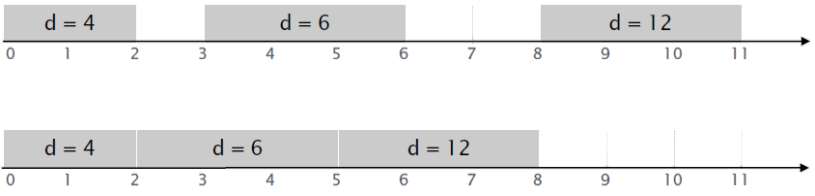
\includegraphics[width=0.67\linewidth]{figures/minimizing-lateness-observation-1.png}
    \end{center}

    \item \textbf{Observation 2:} Earliest deadline first has no idle time.

    \item \textbf{Observation 3:} By definition, earliest deadline first has no inversions.

    There, an inversion is a pair of jobs $i$ and $j$ such that $d_i < d_j$ but $j$ is scheduled before $i$.

    \item \textbf{Observation 4:} If a schedule with no idle time has at least one inversion, it has a pair of inverted jobs scheduled consecutively.

    \item \textbf{Observation 5:} Swapping adjacently scheduled inverted jobs does not increase lateness but reduces the number of inversions by one.

    \begin{center}
        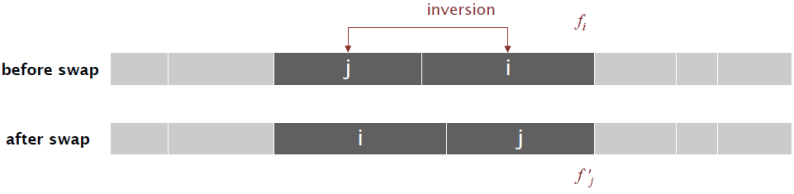
\includegraphics[width=0.67\linewidth]{figures/minimizing-lateness-observation-5.png}
    \end{center}

    \textit{Proof.}
        Let $\ell_k$ and $\ell'_k$ denote the lateness of job $k$ before and after the swap.

        Let $L = \max_k \ell_k$ and $L' = \max_k \ell'_k$ be the maximum lateness.

        Let $i$ and $j$ be the inverted jobs.

        \begin{listu}
            \item $\ell_k = \ell'_k$ for all $k \ne i, j$.

            \item $\ell'_i \le \ell_i$

            \item $\ell'j = f'_j - d_j = f_i - d_j \le f_i - d_i = \ell_i$

            This uses the fact that, due to the inversion, $d_j \ge d_i$.

            \item $\displaystyle L' = \max\left\{\ell'_i, \ell'_j, \max_{k \ne i, j} \ell'_k\right\} \le \max\left\{\ell_i, \ell_j, \max_{k \ne i, j} \ell_k\right\} = L$ \qed
        \end{listu}
\end{listu}

Observations 4 and 5 together is the key to the proof of optimality.

\begin{remark}
    Recall the proof of optimality of the greedy algorithm for interval scheduling

    \begin{listu}
        \item Take an optimal solution matching greedy for $r$ steps, and produced another optimal solution matching greedy for $r + 1$ steps
        \item ``Wrapped'' in a proof by contradiction or proof by induction
    \end{listu}

    Observations 4 and 5 provide a similar structure. If optimal solution does not fully match greedy (the number of inversions $\ge 1$), we can swap an adjacent inverted pair and reduce the number of inversions by one.
\end{remark}

\subsubsection{By Contradiction}

\begin{proof}
    Suppose for contradiction that the greedy EDF solution is not optimal

    \begin{listu}
        \item Consider an optimal schedule $S^*$ with the fewest inversions\footnote{Note that this part is a little flawed, as $S^*$ may be different from the greedy EDF solution based on how we break ties. To fix this, we can simply change the way we break ties until we get the same solution as the greedy EDF solution. Since these jobs are adjacent, we can do this by swapping adjacent jobs, and, by Observation 5, this will not increase the lateness, so the solution remains optimal.}. Without loss of generality, assume it has no idle time.

        \item Since the greedy EDF solution is not optimal, there is at least one inversion in $S^*$.

        \item By Observation 4, the pair of inversion $(i, j)$ are scheduled consecutively (adjacent).

        \item By Observation 5, swapping the adjacent pair keeps the schedule optimal but reduces the number of inversions by 1

        This is a contradiction, as $S^*$ has the fewest inversions.
    \end{listu}

    Thus, the greedy EDF solution is optimal.
\end{proof}

\subsubsection{By Induction}

\begin{proof}
    By induction on the number of inversions in an optimal schedule.

    \begin{claim}
        For each $r \in \left\{ 0, 1, 2, \dots, \binom{n}{2} \right\}$, there is an optimal schedule with at most $r$ inversions.
    \end{claim}

    \begin{listu}
        \item \textbf{Base case:} $r = \binom{n}{2}$

        This is trivially true.

        \item \textbf{Inductive step:} $t + 1 \to t$

        Suppose the claim holds for $t + 1$.

        Take an optimal schedule $S^*$ with at most $t + 1$ inversions.

        Without loss of generality, assume it has no idle time.

        \begin{listu}
            \item If $S^*$ has at most $t$ inversions, we are done.

            \item If $S^*$ has exactly $t + 1$ inversions, then there is a pair of inverted jobs $(i, j)$ scheduled consecutively by Observation 4.

            By Observation 5, swapping the adjacent pair keeps the schedule optimal but reduces the number of inversions by 1.

            The number of inversions in the new schedule is at most $t$, and the claim holds.
        \end{listu}
    \end{listu}

    Claim for $r = 0$ shows optimality of the greedy EDF solution.
\end{proof}

\subsubsection{Contradiction vs Induction}

The favour over contradiction or induction is a matter of taste. It may be the case that for some problems, one method is easier to apply than the other. There is no inherent difference in the two methods, as they both make the same claim and use the same key argument, and one does not need to stick to one method. Meanwhile, as we have seen for the interval partitioning problem, sometimes we may require an entirely different method to prove optimality.
\section{Lossless Compression}

\subsection{Problem Definition}

\begin{example}
    We have a document that is written using $n$ distinct labels. The na\"ive encoding would use $\log_2 n$ bits for each label, but it is not optimal. We can assign shorter encodings to more frequent labels.

    {~~~}

    Say we assign $a = 0$, $b = 1$, $c = 01$, $\dots$ based on the frequency of the labels. However, now we have created confusion when decoding, as $01$ can be decoded as either `ab' or `c'.

    {~~~}

    To avoid conflicts, we need a \term{prefix-free encoding}, where no label is a prefix of another label. Now, we can read left to right, and whenever the part to the left becomes a valid encoding, we greedily decode it, and continue with the rest.
\end{example}

\begin{definition}[Lossless Compression]\index{Lossless Compression}\label{def:lossless-compression}
    Given $n$ symbols and their frequencies $(w_1, \dots, w_n)$, find a prefix-tree encoding with length $(\ell_1, \dots, \ell_n)$ assigned to the symbols which minimizes $\displaystyle \sum_{i=1}^n w_i \ell_i$.
\end{definition}

We observe that prefix-free encodings can be represented by a binary tree.

\begin{center}
    \tikzsetnextfilename{huffman}
    \tikzexternalenable
    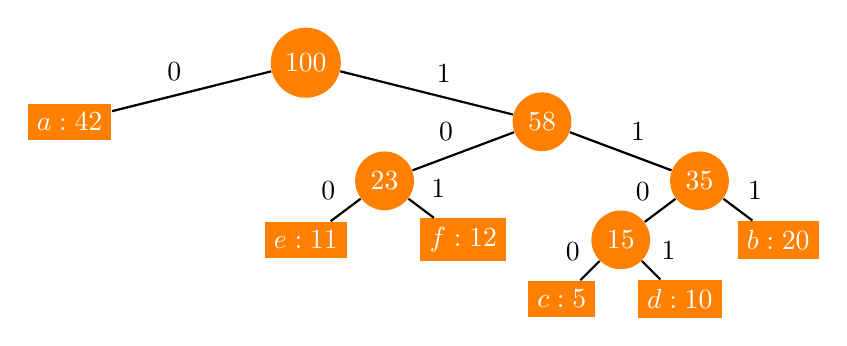
\begin{tikzpicture}[
        inte-node/.style={circle,text=white,fill=orange},
        leaf-node/.style={rectangle,text=white,fill=orange},
        baseline=(current bounding box.north)
    ]
        \node[inte-node] (100) at (0, 0) {$100$};

        \node[leaf-node] (a)  at (-3, -0.75) {$a:42$};
        \node[inte-node] (58) at (3, -0.75) {$58$};

        \node[inte-node] (23) at (1, -1.5) {$23$};
        \node[inte-node] (35) at (5, -1.5) {$35$};

        \node[leaf-node] (e)  at (0, -2.25) {$e:11$};
        \node[leaf-node] (f)  at (2, -2.25) {$f:12$};
        \node[inte-node] (15) at (4, -2.25) {$15$};
        \node[leaf-node] (b)  at (6, -2.25) {$b:20$};

        \node[leaf-node] (c)  at (3.25, -3) {$c:5$};
        \node[leaf-node] (d)  at (4.75, -3) {$d:10$};

        \draw[thick] (100) -- (a) node[midway, above left] {0};
        \draw[thick] (100) -- (58) node[midway, above right] {1};
        \draw[thick] (58) -- (23) node[midway, above left] {0};
        \draw[thick] (58) -- (35) node[midway, above right] {1};
        \draw[thick] (23) -- (e) node[midway, above left] {0};
        \draw[thick] (23) -- (f) node[midway, above right] {1};
        \draw[thick] (35) -- (15) node[midway, above left] {0};
        \draw[thick] (35) -- (b) node[midway, above right] {1};
        \draw[thick] (15) -- (c) node[midway, above left] {0};
        \draw[thick] (15) -- (d) node[midway, above right] {1};
    \end{tikzpicture}
    \tikzexternaldisable
\end{center}

\vspace{-3em}
\subsection{Huffman Encoding}

The Huffman encoding algorithm is a greedy algorithm that generates an optimal prefix-tree encoding for a given set of symbols and their frequencies. 

% \vspace{-1em}
\begin{algorithm}
    \begin{algorithmic}
        \Function{Huffman-Encoding}{$n, w_1, w_2, \dots, w_n$}
            \State $Q \gets \text{Priority-Queue}$
            \For{each symbol $x$}
                \State \Call{Insert}{$Q, x, w_x$}
            \EndFor

            \For{$i = 1$ \To $n - 1$}
                \State $(x, w_x) \gets \text{Extract-Min}(Q)$
                \State $(y, w_y) \gets \text{Extract-Min}(Q)$
                \State \Call{Insert}{$Q, (x, y), w_x + w_y$}
            \EndFor

            \State \Return the root of the tree
        \EndFunction
    \end{algorithmic}
\end{algorithm}

\newpage
\begin{example}
    We use the Huffman encoding algorithm to generate the tree for the previous example.

    \begin{center}
        \tikzexternalenable
        
\begin{tikzpicture}[
            inte-node/.style={circle,text=white,fill=orange},
            leaf-node/.style={rectangle,text=white,fill=orange},
        ]
            \node[leaf-node] (c) at (-5, 0) {$c:5$};
            \node[leaf-node] (d) at (-3, 0) {$d:10$};
            \node[leaf-node] (e) at (-1, 0) {$e:11$};
            \node[leaf-node] (f) at (1, 0) {$f:12$};
            \node[leaf-node] (b) at (3, 0) {$b:20$};
            \node[leaf-node] (a) at (5, 0) {$a:42$};
        \end{tikzpicture}
        \tikzexternaldisable

        \vspace{0.25em} 
\includegraphics[width=2em]{tikz/down-arrow.pdf} \vspace{0.25em}

        \tikzexternalenable
        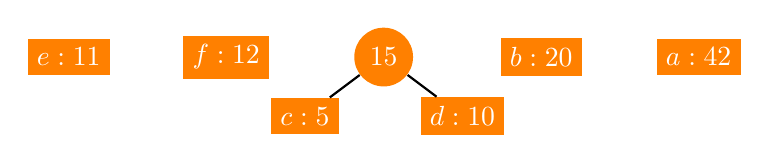
\begin{tikzpicture}[
            inte-node/.style={circle,text=white,fill=orange},
            leaf-node/.style={rectangle,text=white,fill=orange},
        ]
            \node[leaf-node] (e) at (-4, 0) {$e:11$};
            \node[leaf-node] (f) at (-2, 0) {$f:12$};
            \node[leaf-node] (b) at (2, 0) {$b:20$};
            \node[leaf-node] (a) at (4, 0) {$a:42$};

            \node[inte-node] (15) at (0, 0) {$15$};
            \node[leaf-node] (c) at (-1, -0.75) {$c:5$};
            \node[leaf-node] (d) at (1, -0.75) {$d:10$};

            \draw[thick] (15) -- (c);
            \draw[thick] (15) -- (d);
        \end{tikzpicture}
        \tikzexternaldisable

        \vspace{0.25em} 
\includegraphics[width=2em]{tikz/down-arrow.pdf} \vspace{0.25em}

        \tikzexternalenable
        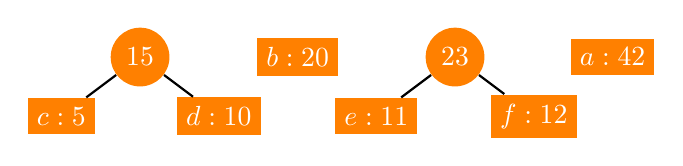
\begin{tikzpicture}[
            inte-node/.style={circle,text=white,fill=orange},
            leaf-node/.style={rectangle,text=white,fill=orange},
        ]
            \node[leaf-node] (b) at (-1, 0) {$b:20$};
            \node[leaf-node] (a) at (3, 0) {$a:42$};

            \node[inte-node] (15) at (-3, 0) {$15$};
            \node[leaf-node] (c) at (-4, -0.75) {$c:5$};
            \node[leaf-node] (d) at (-2, -0.75) {$d:10$};

            \node[inte-node] (23) at (1, 0) {$23$};
            \node[leaf-node] (e) at (0, -0.75) {$e:11$};
            \node[leaf-node] (f) at (2, -0.75) {$f:12$};

            \draw[thick] (15) -- (c);
            \draw[thick] (15) -- (d);
            \draw[thick] (23) -- (e);
            \draw[thick] (23) -- (f);
        \end{tikzpicture}
        \tikzexternaldisable

        \vspace{0.25em} 
\includegraphics[width=2em]{tikz/down-arrow.pdf} \vspace{0.25em}

        \tikzexternalenable
        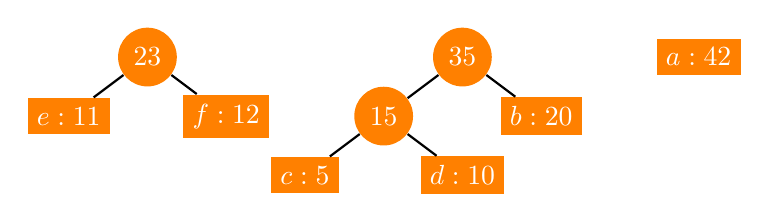
\begin{tikzpicture}[
            inte-node/.style={circle,text=white,fill=orange},
            leaf-node/.style={rectangle,text=white,fill=orange},
        ]
            \node[leaf-node] (a) at (4, 0) {$a:42$};
            
            \node[inte-node] (23) at (-3, 0) {$23$};
            \node[leaf-node] (e) at (-4, -0.75) {$e:11$};
            \node[leaf-node] (f) at (-2, -0.75) {$f:12$};

            \node[inte-node] (35) at (1, 0) {$35$};
            \node[inte-node] (15) at (0, -0.75) {$15$};
            \node[leaf-node] (c) at (-1, -1.5) {$c:5$};
            \node[leaf-node] (d) at (1, -1.5) {$d:10$};
            \node[leaf-node] (b) at (2, -0.75) {$b:20$};

            \draw[thick] (15) -- (c);
            \draw[thick] (15) -- (d);
            \draw[thick] (23) -- (e);
            \draw[thick] (23) -- (f);
            \draw[thick] (35) -- (15);
            \draw[thick] (35) -- (b);
        \end{tikzpicture}
        \tikzexternaldisable

        \vspace{0.25em} 
\includegraphics[width=2em]{tikz/down-arrow.pdf} \vspace{0.25em}

        \tikzexternalenable
        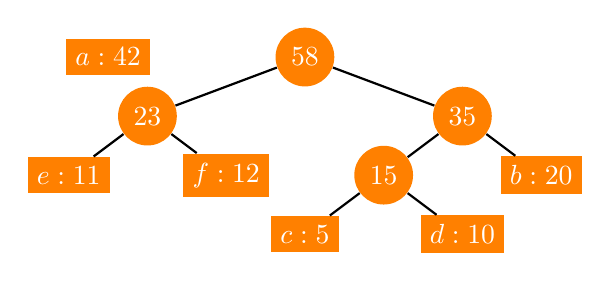
\begin{tikzpicture}[
            inte-node/.style={circle,text=white,fill=orange},
            leaf-node/.style={rectangle,text=white,fill=orange},
        ]
            \node[leaf-node] (a) at (-2.5, 0) {$a:42$};

            \node[inte-node] (58) at (0, 0) {$58$};

            \node[inte-node] (23) at (-2, -0.75) {$23$};
            \node[leaf-node] (e) at (-3, -1.5) {$e:11$};
            \node[leaf-node] (f) at (-1, -1.5) {$f:12$};

            \node[inte-node] (35) at (2, -0.75) {$35$};
            \node[inte-node] (15) at (1, -1.5) {$15$};
            \node[leaf-node] (c) at (0, -2.25) {$c:5$};
            \node[leaf-node] (d) at (2, -2.25) {$d:10$};
            \node[leaf-node] (b) at (3, -1.5) {$b:20$};

            \draw[thick] (15) -- (c);
            \draw[thick] (15) -- (d);
            \draw[thick] (23) -- (e);
            \draw[thick] (23) -- (f);
            \draw[thick] (35) -- (15);
            \draw[thick] (35) -- (b);
            \draw[thick] (58) -- (23);
            \draw[thick] (58) -- (35);
        \end{tikzpicture}

        \vspace{0.25em} 
\includegraphics[width=2em]{tikz/down-arrow.pdf} \vspace{0.25em}

        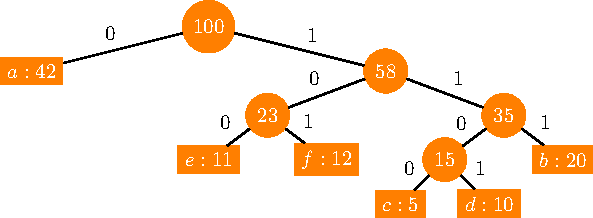
\includegraphics{tikz/huffman.pdf}
    \end{center}
\end{example}

\subsubsection{Running Time}

The running time of the Huffman encoding algorithm is $\mathcal{O}(n \log n)$. However, it can be made $\bigo{n}$ if the labels are sorted by frequency, by using two queues. 

\subsection{Proof of Optimality}

\begin{proof}
    By induction on the number of symbols $n$.

    \begin{listu}
        \item \textbf{Base case:} $n = 2$

        Both encodings which assign 1 bit to each symbol are optimal.

        \item \textbf{Inductive step:} $n - 1 \to n$

        Assume Huffman encoding returns an optimal encoding with $n - 1$ symbols. Consider the case with $n$ symbols.

        \begin{lemma*}[1]\label{lem:huffman-1}
            If $w_x < w_y$, then $\ell_x \ge \ell_y$ in any optimal tree.
        \end{lemma*}

        \begin{proof}
            Proof of \hyperref[lem:huffman-1]{Lemma 1}

            Suppose for contradiction that $w_x < w_y$ and $\ell_x < \ell_y$ in an optimal tree.

            Swapping $x$ and $y$ strictly decreases the total encoding length, as \[
                w_x \cdot \ell_y + w_y \cdot \ell_x < w_x \cdot \ell_x + w_y \cdot \ell_y.
            \]

            This is a contradiction.
        \end{proof}

        Consider the two symbols $x$ and $y$ with lowest frequency which Huffman encoding combines in the first step.

        \begin{lemma*}[2]\label{lem:huffman-2}
            Exists an optimal tree $T$ in which $x$ and $y$ are siblings.

            That is, for some $p$, $x$ and $y$ are assigned encodings of the form $p0$ and $p1$.
        \end{lemma*}

        \textit{Proof.}
            Proof of \hyperref[lem:huffman-2]{Lemma 2}

            \begin{listo}
                \item Let $T$ be an optimal tree.
                \item Let $x$ be the label with the lowest frequency in $T$.
                \item If $x$ does not have the longest encoding in $T$, swap it with the label with the longest encoding.
                \item Due to optimality, $x$ must have a sibling $y'$ (otherwise, we can swap $x$ with its parent and reduce the total encoding length).
                \item If $y'$ is not $y$, swap it with $y$.
                \item We check that Steps 3 and 5 does not change the overall length. \qed
            \end{listo}

        Let $x$ and $y$ be the two least frequency symbols that Huffman combines in the first step into ``$xy$''.

        Let $H$ be the Huffman tree produced. 

        Let $T$ be an optimal tree in which $x$ and $y$ are siblings.

        Let $H'$ and $T'$ be obtained from $H$ and $T$ bt treating $xy$ as one symbol with frequency $w_x + w_y$.

        By the inductive hypothesis, $T'$ is optimal for the $n - 1$ symbols, so $\textsc{Length}(H') \le \textsc{Length}(T')$.

        \begin{listu}
            \item $\textsc{Length}(H) = \textsc{Length}(H') + (w_x + w_y) \cdot 1$
            \item $\textsc{Length}(T) = \textsc{Length}(T') + (w_x + w_y) \cdot 1$
        \end{listu}

        Therefore, $\textsc{Length}(H) \le \textsc{Length}(T)$.
    \end{listu}

    Thus, the Huffman encoding algorithm returns an optimal encoding.
\end{proof}

\section{Other Greedy Algorithms}

Some other greedy algorithms include
\begin{listu}
    \item \textbf{Shortest Path:} Dijkstra's algorithm
    \item \textbf{Minimum Spanning Tree:} Kruskal's algorithm and Prim's algorithm
\end{listu}
\chapter{Dynamic Programming}
\vspace{-1em}
\begin{center}
    \begin{minipage}[t]{0.8\linewidth}
        \textit{Everyone should tattoo the following sentence on the back of their hands, right under all the rules about logarithms and big-Oh notation:}
    \end{minipage}

    {~~~}

    \vspace{0.5em}
    
\includegraphics[width=0.45\linewidth]{figures/greedy-never-works.png}
    \begin{flushright}
        --- \textit{Jeff Erickson, \textbf{Algorithms}}
    \end{flushright}
\end{center}

\section{Introduction}

\term{Dynamic programming}\index{Dynamic Programming} was developed by Richard Bellman in the 1950s, and is both a mathematical optimization method and a computer programming method. It is a method for solving complex problems by breaking them down into simpler subproblems, similar to the divide-and-conquer method, with the added benefit of storing the results of subproblems so that they are not recomputed. It is also more powerful than divide-and-conquer, as it can be used to solve problems where subproblems overlap.

\begin{itemize}
    \item Breaking the problem down into simpler subproblems, solve each subproblem just once, and store their solutions. 
    \item The next time the same subproblem occurs, instead of recomputing its solution, simply look up its previously computed solution.
    \item Hopefully, we save a lot of computation at the expense of modest increase in storage space. 
    \item Also called ``\bred{memoization}''.
\end{itemize}

\section{Weighted Interval Scheduling}

\subsection{Problem Definition}

\begin{itemize}
    \item Job $j$ starts at time $s_j$ and finishes at time $f_j$.
    \item Each job $j$ has a weight $w_j$.
    \item Two jobs $i$ and $j$ are compatible if $f_i \leq s_j$.
    \item \textbf{Goal:} find a set $S$ of mutually compatible jobs that maximizes $\sum_{j \in S} w_j$.
\end{itemize}

If all the weights are equal, this is the same as the \hyperref[sec:interval-scheduling]{\textbf{interval scheduling}} problem. However, if the weights are not equal, the greedy algorithm for interval scheduling fails spectacularly.

\begin{center}
    \tikzexternalenable
    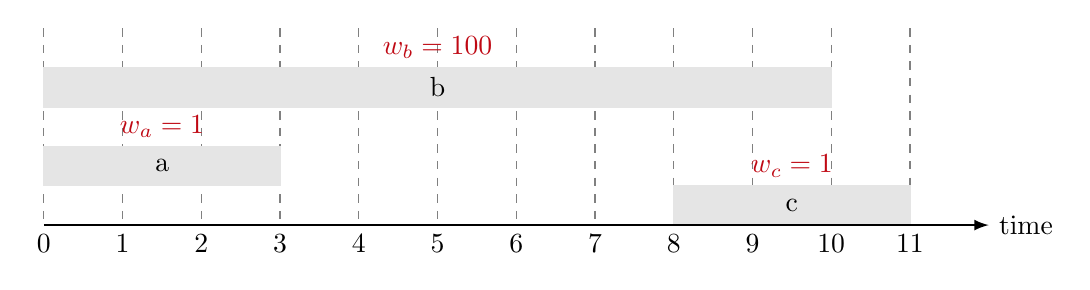
\begin{tikzpicture}
        \definecolor{light-gray}{gray}{0.9}
        \foreach \x in {0, 1, 2, 3, 4, 5, 6, 7, 8, 9, 10, 11}
            \draw[gray,dashed] (\x, 2.5) -- (\x, 0) node[black,below] {\x};

        \draw[light-gray,fill] (0, 0.5) rectangle (3, 1)    node[black,midway] {a};
        \draw[light-gray,fill] (0, 1.5) rectangle (10, 2)   node[black,midway] {b};
        \draw[light-gray,fill] (8, 0)   rectangle (11, 0.5) node[black,midway] {c};

        \draw[thick,-latex] (0, 0) -- (12, 0) node[right] {time};

        \node[darkRed] at (1.5, 1.25) {$w_a = 1$};
        \node[darkRed] at (5, 2.25)   {$w_b = 100$};
        \node[darkRed] at (9.5, 0.75) {$w_c = 1$};
    \end{tikzpicture}
    \tikzexternaldisable
\end{center}

What if we use other orderings? We can order the jobs by weight and choose the one with the highest $w_j$ first, or we can order by maximum weight per time, and select jobs with the highest $w_j / (f_j - s_j)$ first. However, none of these orderings work. They are arbitrarily worse than the optimal solution. 

\subsubsection{Convention}

\begin{itemize}
    \item Jobs are sorted by finish time: $f_1 \leq f_2 \leq \ldots \leq f_n$.
    \item $p[j] = \max\{i: i < j \text{ and } f_i < s_j\}$, the largest $i < j$ such that job $i$ is compatible with job $j$.
    \begin{itemize}
        \item Jobs $1, \dots, i$ are compatible with $j$, but jobs $i + 1, \dots j - 1$ are not.
        \item $p[j]$ can be computed via binary search in $O(\log n)$ time.
    \end{itemize}
\end{itemize}

\subsection{Dynamic Programming Solution}

\begin{itemize}
    \item Let OPT be an optimal solution to the problem.

    \item There are two options for job $n$:

    \begin{itemize}
        \item Job $n$ is in OPT

        We cannot use the incompatible jobs $\{ p[n] + 1, \dots, n - 1 \}$

        Must select the optimal solution for the remaining jobs $\{1, \dots, p[n]\}$.

        \item Job $n$ is not in OPT

        Must select the optimal solution for the remaining jobs $\{1, \dots, n - 1\}$.
    \end{itemize}

    \item OPT is the best of these two options.

    Notice that in both options, we need to solve the problem on a prefix of our ordering.

    \item Let $OPT(j)$ be the maximum total weight of compatible jobs from $\{1, \dots, j\}$.

    \item \textbf{Base case:} $OPT(0) = 0$.

    \item \textbf{Recurrence:} $OPT(j) = \max\{w_j + OPT(p[j]), OPT(j - 1)\}$.

    \begin{itemize}
        \item Job $j$ is selected: optimal weight is $w_j + OPT(p[j])$.
        \item Job $j$ is not selected: optimal weight is $OPT(j - 1)$.
    \end{itemize}

    The \term{Bellman equation} is \[
        OPT(j) = \begin{cases}
            0                                   & \text{if } j = 0 \\
            \max\{w_j + OPT(p[j]), OPT(j - 1)\} & \text{if } j > 0
        \end{cases}
    \]
\end{itemize}

\newpage
\begin{example}[Brute Force Solution]
    Below is a brute force solution to the problem. 

    \begin{algorithm}[ht!]
        \begin{algorithmic}[1]
            \Function{Brute-Force}{$n, s_1, \dots, s_n, f_1, \dots, f_n, w_1, \dots, w_n$}
                \State Sort jobs by finish time and renumber so that $f_1 \leq f_2 \leq \ldots \leq f_n$.
                \State Compute $p[1], \dots, p[n]$ via binary search.
                \State \Return \Call{Compute-Opt}{$n$}
            \EndFunction

            {~~~}

            \Function{Compute-Opt}{$j$}
                \If{$j = 0$}
                    \State \Return 0
                \Else
                    \State \Return $\max\{w_j + \Call{Compute-Opt}{p[j]}, \Call{Compute-Opt}{j - 1}\}$
                \EndIf
            \EndFunction
        \end{algorithmic}
    \end{algorithm}

    Note that \textsc{Compute-Opt} has a time complexity of $O(2^n)$, which is extremely inefficient. This is because some solutions are being computed multiple times. For example, \textsc{Compute-Opt}$(j - 1)$ is computed multiple times. For example, if $p[5] = 3$, then \textsc{Compute-Opt}$(3)$ is computed twice: once for $j = 4$ and once for $j = 5$.

    To imporve, we can simply remember the results of subproblems and look them up when needed.
\end{example}

Let's store \textsc{Store-Opt}$(j)$ in an array $M[j]$.

\subsubsection{Top-Down Dynamic Programming}

\begin{algorithm}[ht!]
    \begin{algorithmic}[1]
        \Function{Top-Down}{$n, s_1, \dots, s_n, f_1, \dots, f_n, w_1, \dots, w_n$}
            \State Sort jobs by finish time and renumber so that $f_1 \leq f_2 \leq \ldots \leq f_n$.
            \State Compute $p[1], \dots, p[n]$ via binary search.
            \State $M[0] \gets 0$.
            \State \Return \Call{M-Compute-Opt}{$n$}
        \EndFunction

        {~~~}

        \Function{M-Compute-Opt}{$j$}
            \If{$M[j]$ is ininitialized}
                \State $M[j] \gets \max\{w_j + \Call{Store-Opt}{p[j]}, \Call{Store-Opt}{j - 1}\}$
            \EndIf
            \State \Return $M[j]$
        \EndFunction
    \end{algorithmic}
\end{algorithm}

\begin{claim}
    This memoized version takes $\mathcal{O}(n \log n)$ time.
\end{claim}

\begin{itemize}
    \item Sorting by finish time takes $\mathcal{O}(n \log n)$ time.
    \item Computing $p[1], \dots, p[n]$ takes $\mathcal{O}(n \log n)$ time.
    \item For each $j$, at most one of the calls to \textsc{M-Compute-Opt}$(j)$ will make two recursive calls.
    \begin{itemize}
        \item At most $\mathcal{O}(n)$ total calls to \textsc{M-Compute-Opt}.
        \item Each call takes $\mathcal{O}(1)$ time, not considering the time spent in the recursive calls. 
        \item Hence, the initial call, \textsc{M-Compute-Opt}$(n)$, finished in $\mathcal{O}(n)$ time.
    \end{itemize}
\end{itemize}

\subsubsection{Bottom Up Dynamic Programming}

In bottom up dynamic programming, we need to find an order in which to call the functions so that the subsolutions are ready when needed. However, this is generally more efficient, as it avoids the overhead of recursion.

\begin{algorithm}[ht!]
    \begin{algorithmic}[1]
        \Function{Bottom-Up}{$n, s_1, \dots, s_n, f_1, \dots, f_n, w_1, \dots, w_n$}
            \State Sort jobs by finish time and renumber so that $f_1 \leq f_2 \leq \ldots \leq f_n$.
            \State Compute $p[1], \dots, p[n]$ via binary search.
            \State $M[0] \gets 0$.
            \For{$j = 1$ to $n$}
                \State $M[j] \gets \max\{w_j + M[p[j]], M[j - 1]\}$
            \EndFor
            \State \Return $M[n]$
        \EndFunction
    \end{algorithmic}
\end{algorithm}

\subsubsection{Top-Down vs. Bottom-Up}

\begin{itemize}
    \item Top-Down may be preferred\dots
    \begin{itemize}
        \item {\dots}when not all sub-solutions need to be computed on some inputs
        \item {\dots}because one does not need to think of the ``right order'' in which to compute sub-solutions
    \end{itemize}

    \item Bottom-Up may be preferred\dots
    \begin{itemize}
        \item {\dots}when all sub-solutions will anyway need to be computed
        \item {\dots}because it is faster as it prevents recursive call overheads and unnecessary random memory accesses
        \item {\dots}because sometimes we can free-up memory early
    \end{itemize}
\end{itemize}

\subsubsection{Optimal Solution Reconstruction}

So far, we have only computed the maximum total weight of compatible jobs. We have not yet computed the set of jobs that achieves this maximum. To do so, we can simply store the choices made in the Bellman equation. So, we compute two quantities \[
    OPT(j) = \begin{cases}
        0                                   & \text{if } j = 0 \\
        \max\{w_j + OPT(p[j]), OPT(j - 1)\} & \text{if } j > 0
    \end{cases}
\] and \[
    S(j) = \begin{cases}
        \varnothing & \text{if } j = 0                                             \\
        S(j - 1)    & \text{if } j > 0 \text{ and } OPT(j - 1) \ge w_j + OPT(p[j]) \\
        \{j\}       & \text{if } j > 0 \text{ and } OPT(j - 1) < w_j + OPT(p[j])
    \end{cases}
\]

This works with both top-down and bottom-up implementations. We can compute OPT and $S$ simultaneously, or compute $S$ after computing OPT. 

{~~~}

One may notice that this implementation is wasting a lot of space. We are copying the entire solution of $S(j - 1)$ to $S(j)$, which is a by-element array copy. We can avoid this by only storing the change in the solution, \[
    S(j) = \begin{cases}
        \perp & \text{if } j = 0                                             \\
        L     & \text{if } j > 0 \text{ and } OPT(j - 1) \ge w_j + OPT(p[j]) \\
        R     & \text{if } j > 0 \text{ and } OPT(j - 1) < w_j + OPT(p[j])
    \end{cases}
\] where we store only one bit of information for each $j$: which option yielded the maximum weight. 

To reconstruct the optimal solution, start with $j = n$:
\begin{itemize}
    \item If $S(j) = L$, update $j \gets j - 1$.
    \item If $S(j) = R$, add job $j$ to the solution and update $j \gets p[j]$.
    \item If $S(j) = \perp$, stop.
\end{itemize}

\subsection{Optimal Substructure Property}

Dynamic programming applies well to problems that have optimal substructure property. That is, the optimal solution to a problem can be computed easily given optimal solution to subproblems.

\begin{remark}
    Recall that divide-and-conquer also uses this property. It is a special case in which the subproblems do not ``overlap'', so, there is no need for memoization.

    In dynamic programming, two of the subproblems may in turn require access to solution to the same subproblem.
\end{remark}

\section{Knapsack Problem}

\subsection{Problem Definition}

\begin{itemize}
    \item There are $n$ items, each provides a value $v_i > 0$ and a weight $w_i > 0$.
    \item There is a knapsack that can hold a maximum weight of $W$.
    \item Assume that $W, v_i$-s, and $w_i$-s are all integers.
    \item \textbf{Goal:} pack the knapsack with a subset of items with highest total value subject to their total weight being at most $W$. 
\end{itemize}

\subsection{Dynamic Programming Solution}

\begin{itemize}
    \item Let $OPT(i, w)$ be the maximum value we can pack using only items $1, \dots, i$ in s knapsack of capacity $w$.
    
    \textbf{Goal:} compute $OPT(n, W)$.

    \item Consider item $i$ 
    
    \begin{itemize}
        \item If $w_i > w$, then we can't choose $i$. Use $OPT(i - 1, w)$.
        \item If $w_i \leq w$, then we have two options:
        \begin{itemize}
            \item If we choose $i$, then the best value is $v_i + OPT(i - 1, w - w_i)$.
            \item If we don't choose $i$, then the best value is $OPT(i - 1, w)$.
        \end{itemize}
    \end{itemize}
\end{itemize} 

\[
    OPT(i, w) = \begin{cases}
        0                                                & \text{if } i = 0   \\
        OPT(i - 1, w)                                    & \text{if } w_i > w \\
        \max\{v_i + OPT(i - 1, w - w_i), OPT(i - 1, w)\} & \text{otherwise}
    \end{cases}
\]

\subsubsection{Running Time}

Consider the possible evaluations of $OPT(i, w)$
\begin{itemize}
    \item $i \in \{ 1, \dots, n \}$
    \item $w \in \{ 0, \dots, W \}$
    \item There are $\mathcal{O}(n \cdot W)$ possible evaluations of $OPT(i, w)$.

    Each is computed in $\mathcal{O}(1)$ time, at most once. 

    \item The total running time is $\mathcal{O}(n \cdot W)$.
\end{itemize}

This is a \term{pseudo-polynomial time} algorithm. The time is not polynomial in \[ \log W + \sum_{i=1}^n (\log v_i + \log w_i), \] the number of bits required to represent the input, but it is polynomial in the numeric value of the input in unary representation.

\begin{definition}[Pseudo-Polynomial Time Algorithm]\index{Pseudo-Polynomial Time Algorithm}\label{def:pseudo-polynomial-time-algorithm}
    An algorithm is \term{pseudo-polynomial time} if its running time is polynomial in the numeric value of the input in unary representation, but not in the number of bits required to represent the input.
\end{definition}

\begin{definition}[Unary Representation]\index{Unary Representation}\label{def:unary-representation}
    A number is in \term{unary representation} if it is represented as a sequence of 1's. For example, the number 5 is represented as 11111.
\end{definition}

\begin{remark}
    For the knapsack problem, the number of bits required to represent the input is \[
        T = \log W + \sum_{i=1}^n (\log v_i + \log w_i).
    \]

    Running time of the dynamic programming solution is $\mathcal{O}(n \cdot W)$. If $W$ takes the form $2^n$, then $T \in \mathcal{O}(n)$, but the running time is $\mathcal{O}(n \cdot 2^n)$. There is no way to $n \cdot 2^n$ as a polynomial in $n$.

    {~~~}

    However, if we consider the unary representation of the input, then \[ T = W + \sum_{i=1}^n (v_1 + w_1). \] We know that $T \ge n$ and $T \ge W$, so the running time $\mathcal{O}(n \cdot W) = \mathcal{O}(T^2)$ is polynomial in $T$.
\end{remark}

\subsubsection{Another Dynamic Programming Solution}

In this solution, we will focus on the values instead of the weights.

\begin{itemize}
    \item Let $OPT(i, v)$ be the minimum weight we need to achieve a value of at least $v$ using only items $1, \dots, i$.

    \textbf{Goal:} compute $OPT(n, V)$, where $V = \sum_{i=1}^n v_i$.

    \item Consider item $i$.

    \begin{itemize}
        \item If we choose $i$, then the best weight is $w_i + OPT(i - 1, v - v_i)$.
        \item If we don't choose $i$, then the best weight is $OPT(i - 1, v)$.
    \end{itemize}
\end{itemize} \[
    OPT(i, v) = \begin{cases}
        0                                                & \text{if } i = 0   \\
        OPT(i - 1, v)                                    & \text{if } v_i > v \\
        \min\{w_i + OPT(i - 1, v - v_i), OPT(i - 1, v)\} & \text{otherwise}
    \end{cases}
\]

This approach has a running time of $\mathcal{O}(n \cdot V)$, which is also pseudo-polynomial time.

% TODO: FPTAS

\section{Single-Source Shortest Paths}

\subsection{Problem Definition}

\begin{itemize}
    \item A directed graph $G = (V, E)$ with edge lengths $\ell_{vw}$ on each edge $(v, w)$, and s source vertex $s$.
    \item \textbf{Goal:} compute the shortest path from $s$ to every other vertex $t$.
\end{itemize}

When $\ell_{vw} \ge 0$ for all edges, we can use \hyperref[subsec:dijkstras-algorithm]{Dijkstra's algorithm}. However, when $\ell_{vw}$ can be negative, Dijkstra's algorithm does not work. 

\begin{example}
    Consider when we have a cycle of negative length. In this case, we can keep going around the cycle to get a path of arbitrarily small length.

    In this case, the shortest paths are not well-defined.
\end{example}

To avoid this issue, we need to restrict the graph to avoid negative cycles.

\begin{claim}
    With no negative cycles, there is always a shortest path from any vertex to any other vertex that is \bred{simple}.
\end{claim}

\begin{proof}
    Consider the shortest path from $s$ to $t$ with the fewest edges among all shortest $s \leadsto t$ paths.

    If it has a cycle, removing the cycle creates a path with fewer edges that is no longer than the original path
\end{proof}

\subsection{Dynamic Programming Solution}

\subsubsection{Optimal Substructure Property}

Consider a simple shortest path $P$ from $s$ to $t$.

\begin{itemize}
    \item It could be just a single edge. But if $P$ has more than one edges, consider $u$ which immediately precedes $t$ in the path. 
    \item If $s \leadsto t$ is the shortest, $s \leadsto u$ must also be the shortest, and it must use one fewer edge than $s \leadsto t$.
\end{itemize}

Let $OPT(t, i)$ be the length of the shortest path from $s$ to $t$ using at most $i$ edges. Then,
\begin{itemize}
    \item Either this path uses at most $i - 1$ edges, so $OPT(t, i) = OPT(t, i - 1)$, or
    \item It uses $i$ edges, so $\displaystyle OPT(t, i) = \min_{u} OPT(u, i - 1) + \ell_{ut}$.
\end{itemize} \[
    OPT(t, i) = \begin{cases} 
        0                                                                     & \text{if } i = 0 \text{ or } t = s    \\
        \infty                                                                & \text{if } i = 0 \text{ and } t \ne s \\
        \displaystyle
        \min\left\{ OPT(t, i - 1), \min_{u} OP(u, i - 1) + \ell_{ut} \right\} & \text{otherwise}
    \end{cases}
\]

\subsubsection{Running Time}

There are $\mathcal{O}(n^2)$ entries to evaluate, and each entry takes $\mathcal{O}(n)$ time to evaluate. Hence, the running time is $\mathcal{O}(n^3)$.

\subsection{All-Pairs Shortest Paths}

\subsubsection{Problem Definition}

\begin{itemize}
    \item A directed graph $G = (V, E)$ with edge lengths $\ell_{vw}$ on each edge $(v, w)$.
    \item \textbf{Goal:} compute the shortest path from every vertex $s$ to every other vertex $t$.
\end{itemize}

An na\"ive approach may be to run the previous algorithm for each vertex $s$. However, this approach has a running time of $\mathcal{O}(n^4)$, while it is possible to solve the problem in $\mathcal{O}(n^3)$ time.

Let $OPT(u, v, k)$ be the length of the shortest simple path from $u$ to $v$ using only vertices in $\{1, \dots, k\}$ as intermediate vertices. Then, \[
    OPT(u, v, k) = \begin{cases}
        \ell_{uv}                                                     & \text{if } k = 0 \\
        \min\{OPT(u, v, k - 1), OPT(u, k, k - 1) + OPT(k, v, k - 1)\} & \text{otherwise}
    \end{cases}
\]

\section{Chain Matrix Product}

\subsection{Problem Definition}

\begin{itemize}
    \item Given matrices $M_1, \dots, M_n$, where the dimensions of $M_i$ are $d_{i - 1} \times d_i$.
    \item \textbf{Goal:} compute the product $M_1 \cdot M_2 \cdot \dots \cdot M_n$. 
\end{itemize}

We know that matrix multiplication is associative, so the order of multiplication does not matter. However, the number of scalar multiplications required to compute the product does depend on the order of multiplication. Assume we use the brute force approach for matrix multiplication. Multiplying $p \times q$ and $q \times r$ matrices requires $p \cdot q \cdot r$ scalar multiplications.

\textbf{Note:} Our input is simply the dimensions $d_0, d_1, \dots , d_n$ (such that each $M_i$ is $d_{i-1} \times d_i$) and not the actual matrices

\subsection{Dynamic Programming Solution}

\subsubsection{Optimal Substructure}

We can use dynamic programming to solve this problem, as it has the optimal substructure property.
\begin{itemize}
    \item Think of the final product computed, say $A \cdot B$
    \item $A$ is the product of some prefix, $B$ is the product of the remaining suffix
    \item For the overall optimal computation, each of $A$ and $B$ should be computed optimally
\end{itemize}


Let $OPT(i, j)$ be the minimum number of scalar multiplications required to compute the product $M_i \cdot M_{i + 1} \cdot \dots \cdot M_j$. Then, \[
    OPT(i, j) = \begin{cases}
        0                                                                 & \text{if } i = j \\
        \displaystyle
        \min_{i \leq k < j} \{OPT(i, k) + OPT(k + 1, j) + d_{i - 1} \cdot d_k \cdot d_j\} & \text{if } i < j
    \end{cases}
\]

\subsubsection{Running Time}

There are $\mathcal{O}(n^2)$ entries to evaluate, and each entry takes $\mathcal{O}(n)$ time to evaluate. Hence, the running time is $\mathcal{O}(n^3)$.

\section{Edit Distance}

\subsection{Problem Definition}

This is also known as the sequence alignment problem. We ask how similar are string $X = x_1 x_2 \dots x_m$ and $Y = y_1 y_2 \dots y_n$.

Suppose we can {\color{lightBlue}delete} or {\color{darkGreen}replace} symbols, and can do these operations on any symbol in either string. We want to find the minimum number of operations required to match the two strings.

\begin{example}
    Consider \texttt{ocurrance} and \texttt{occurrence}.

    \begin{figure}[ht!]
        \centering
        \begin{subfigure}[ht!]{0.33\linewidth}
            \centering
            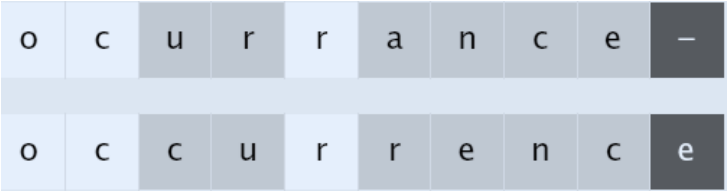
\includegraphics[width=\linewidth]{figures/edit-distance-example-1.png}
            \caption{6 replacements, 1 deletion}
        \end{subfigure}
        \hfil%
        \begin{subfigure}[ht!]{0.33\linewidth}
            \centering
            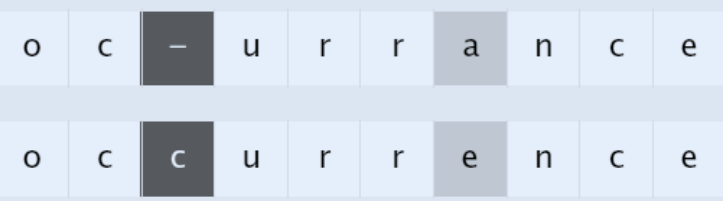
\includegraphics[width=\linewidth]{figures/edit-distance-example-2.png}
            \caption{1 replacement, 1 deletion}
        \end{subfigure}
    \end{figure}
\end{example}

\begin{itemize}
    \item \textbf{input}

    \begin{itemize}
        \item Strings $X = x_1 x_2 \dots x_m$ and $Y = y_1 y_2 \dots y_n$.
        \item Cost $d(a)$ of deleting symbol $a$.
        \item Cost $r(a, b)$ of replacing symbol $a$ with symbol $b$.
        
        We assume $r(a, b) = r(b, a)$ and $r(a, a) = 0$, for all $a, b$.
    \end{itemize}

    \item \textbf{Goal}

    Compute the minimum total cost for matching $X$ and $Y$.
\end{itemize}

\subsection{Dynamic Programming Solution}

\subsubsection{Optimal Substructure}

\begin{itemize}
    \item \textbf{Goal:} match $x_1, \dots, x_m$ with $y_1, \dots, y_n$.

    \item Consider the last symbols $x_m$ and $y_n$.

    \item There are three options:
    
    \begin{itemize}
        \item {\color{lightBlue}Delete} $x_m$, and optimally match $x_1, \dots, x_{m - 1}$ with $y_1, \dots, y_n$.
        \item {\color{lightBlue}Delete} $y_n$, and optimally match $x_1, \dots, x_m$ with $y_1, \dots, y_{n - 1}$.
        \item {\color{darkGreen}Match} $x_m$ and $y_n$, and optimally match $x_1, \dots, x_{m - 1}$ with $y_1, \dots, y_{n - 1}$.
        \begin{itemize}
            \item We increase the cost by $r(x_m, y_n)$ if $x_m \ne y_n$.
            \item Recall that $r(a, a) = 0$, so we don't increase the cost if $x_m = y_n$.
        \end{itemize}
    \end{itemize}

    \item Hence in the dynamic programming, we need to compute the optimal solutions for matching prefixes of $X$ and $Y$, $x_1, \dots, x_i$ and $y_1, \dots, y_j$.
\end{itemize}

Let $E[i, j]$ be the distance between $x_1, \dots, x_i$ and $y_1, \dots, y_j$. Then, \[
    E[i, j] = \begin{cases}
        0                 & \text{if } i = 0 \text{ and } j = 0 \\
        B                 & \text{if } i = 0 \text{ and } j > 0 \\
        A                 & \text{if } i > 0 \text{ and } j = 0 \\
        \min\{ A, B, C \} & \text{otherwise}
    \end{cases}
\] where \[
    \begin{aligned}
        A & = d(x_i) + E[i - 1, j]          \\
        B & = d(y_j) + E[i, j - 1]          \\
        C & = r(x_i, y_j) + E[i - 1, j - 1]
    \end{aligned}
\]

\subsubsection{Running Time}

There are $\mathcal{O}(m \cdot n)$ entries to evaluate, and each entry takes $\mathcal{O}(1)$ time to evaluate. Hence, the running time is $\mathcal{O}(m \cdot n)$.

\subsubsection{Space Optimization}

The current solution uses $\mathcal{O}(m \cdot n)$ space. However, we can optimize the space complexity of the dynamic programming solution by using a bottom up approach. 

\begin{itemize}
    \item While computing $E[\cdot,j]$, we only need to store $E[\cdot,j]$ and $E[\cdot,j-1]$, so the additional space required is $\mathcal{O}(m)$.
    \item By storing two rows at a time instead, we can make it $\mathcal{O}(n)$.
    \item Usually, we include the storage of inputs, so both are $\mathcal{O}(m + n)$.
\end{itemize}

However, this is not enough if we want to compute the actual solution. \href{https://en.wikipedia.org/wiki/Hirschberg%27s_algorithm}{Hirschberg's algorithm} is a space-optimized version of the dynamic programming solution that can compute the actual solution in $\mathcal{O}(m + n)$ space.

% TODO: Hirschberg's algorithm

\section{The Traveling Salesman Problem}

\subsection{Problem Definition}

\begin{itemize}
    \item A complete graph $G = (V, E)$ with distance $d_{i, j}$ from vertex $i$ to vertex $j$.
    
    Note that the input needs to satisfy the triangle inequality: $d_{i, j} \le d_{i, k} + d_{k, j}$ for all $i, j, k$.

    \item \textbf{Goal:} find the shortest cycle that visits every vertex exactly once. This is called the \term{Hamiltonian cycle}.
\end{itemize}

We start at node $v_1 = 1$, and want to visit other nodes in some order, say $v_2, v_3, \dots, v_n, v_1$. The total distance is \[
    d_{1, v_2} + d_{v_2, v_3} + \dots + d_{v_{n-1}, v_n} + d_{v_n, 1},
\] and we want to minimize this.

The na\"ive approach is to consider all possible Hamiltonian cycles and choose the shortest one. However, this approach has a running time of $(n - 1)! = \theta\left( \sqrt{n} \left( \frac{n}{e} \right)^n \right)$ by Stirling's approximation, which is not feasible for large $n$.

\subsection{Dynamic Programming Solution}

Consider $v_n$, the last node before returning to $v_1 = 1$. If $v_n$ is some node $c$, we find the optimal order of visiting nodes $2, 3, \dots, n$ that ends at $c$. To do so, we need to keep track of the subset of nodes visited so far, and the last node visited.

{~~~}

Let $OPT[S, c]$ bethe minimum total travel distance when starting at $1$, visiting each node in $S$ exactly once, and ending at $c \in S$. We can find the best ending node $c$ by computing \[
    \min_{c \in S} \{ OPT[S, c] + d_{c,1} \} \qquad \text{where } S = \{2, 3, \dots, n\}.
\] The Bellman equation is \[
    OPT[S, c] = \begin{cases}
        d_{1, c}                                                                & \text{if } S = \{ c \} \\
        \displaystyle
        \min_{m \in S \setminus \{c\}} ( OPT[S \setminus \{c\}, m] + d_{m, c} ) & \text{if } |S| > 1     \\
    \end{cases}
\] which yields the optimal solution \[
    \text{Final solution} = \min_{c \in \{ 2, \dots, n \}} \{ OPT[{2, \dots, n}, c] + d_{c, 1} \}.
\]

\subsubsection{Running Time}

There are $\mathcal{O}(n \cdot 2^n)$ entries to evaluate, and each entry takes $\mathcal{O}(n)$ time to evaluate. Hence, the running time is $\mathcal{O}(2^n \cdot n^2)$.

\subsection{Space Optimization}

The space complexity of the dynamic programming solution is $\mathcal{O}(n \cdot 2^n)$, which is the same as implementing the solution na\"ively. However, we can optimize by using a bottom up approach, as we do not need the entire table at any given time -- computing the optimal solution with $|S| = k$ only requires storing the optimal solution with $|S| = k - 1$. By doing so, we can reduce the space complexity to approximately \[
    \mathcal{O} \left( n \cdot \binom{n}{n/2} \right) \approx \mathcal{O} \left( \sqrt{n} \cdot 2^n \right).
\]

\section{Remarks}

High-level steps in designing a DP algorithm
\begin{itemize}
    \item Focus on a single decision in optimal solution. Typically, this is the first or the last decision. 

    \item For each possible way of making that decision, [optimal substructure] write the optimal solution of the problem in terms of the optimal solutions to subproblems

    \item Generalize the problem by looking at the type of subproblems needed. 
    
    For example, in the edit distance problem, we realize that we need to solve the problem for prefixes $(x_1, \dots, x_i)$ and $(y_1, \dots , y_j)$ for all $(i,j)$

    \item Write the Bellman equation, cover your base cases 

    \item Think about optimizing the running time/space using tricks. This is often easier in the bottom-up implementation
\end{itemize}
\chapter{Network Flow}

\section{Network Flow Problem}

\begin{itemize}
    \item \textbf{Input:}

    \begin{itemize}
        \item A direct graph $G = (V, E)$
        \item A capacity function $c: E \to \mathbb{R}_{\ge0}$
        \item The source $s \in V$ and the sink $t \in V$
    \end{itemize}

    \item \textbf{Output:} The maximum flow from $s$ to $t$
\end{itemize}

In a network flow problem, we assume
\begin{itemize}
    \item No edges enter $s$
    \item No edges leave $t$
    \item Edge capacity $c(e)$ is a non-negative integer
\end{itemize}

\begin{definition}[Flow]\index{Flow}\label{def:flow}
    An \term{$s-t$ flow} in a network is a function $f: E \to \mathbb{R}_{\ge 0}$ that satisfies the following properties:
    \begin{itemize}
        \item \textbf{Capacity constraint:} For all $e \in E$, \[ 0 \leq f(e) \leq c(e) \]
        \item \textbf{Flow conservation:} For all $v \in V \setminus \{s, t\}$, \[ \sum_{(v, u) \in E} f(v, u) = \sum_{(u, v) \in E} f(u, v) \]
    \end{itemize}

    Intuitively, $f(e)$ is the amount of flow that is sent through edge $e$.
\end{definition}

\begin{figure}[ht!]
    \centering
    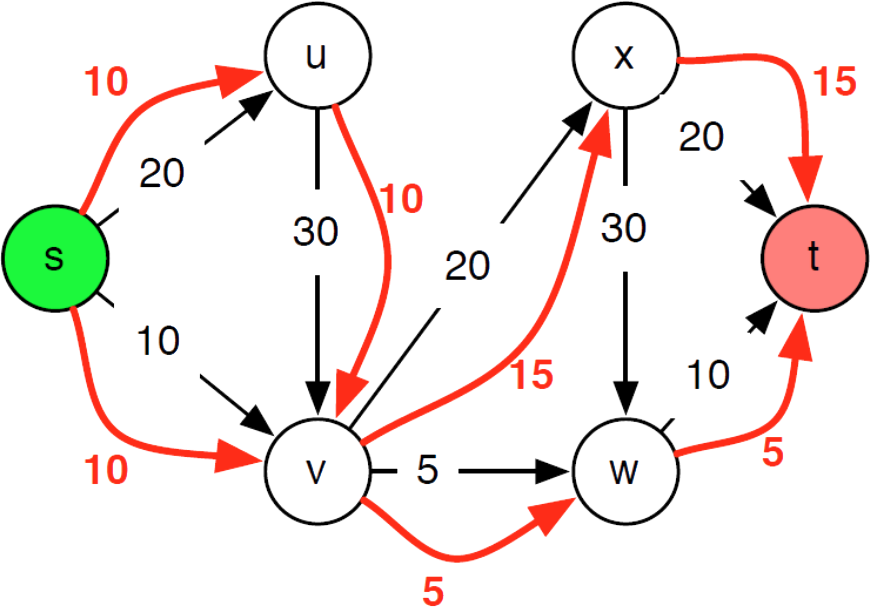
\includegraphics[width=0.33\linewidth]{figures/flow-definition.png}
\end{figure}

\begin{remark}[Notation]
    We define the function \[
        f^{in}(v) = \sum_{(u, v) \in E} f(u, v)
    \] to be the total flow into $v$, and \[
        f^{out}(v) = \sum_{(v, u) \in E} f(v, u)
    \] to be the total flow out of $v$.
\end{remark}

The value of the flow $f$ is defined as \[
    v(f) = f^{out}(s) = f^{in}(t)
\]

\begin{definition}[Network Flow Problem]\index{Network Flow Problem}\label{def:network-flow-problem}
    Given a network $G = (V, E)$, a capacity function $c: E \to \mathbb{R}_{\ge0}$, and two vertices $s, t \in V$, the \term{network flow problem} is to find an $s-t$ flow $f^*$ of maximum value.
\end{definition}

We can try to solve this problem using a greedy algorithm, but it doesn't always work -- once it increases the flow on an edge, it is not allowed to decrease it later. We need a way to ``undo'' the flow on an edge if it turns out to be a bad idea. To do so, we can send some flow \bred{backwards} along the same path.

\begin{figure}[ht!]
    \centering
    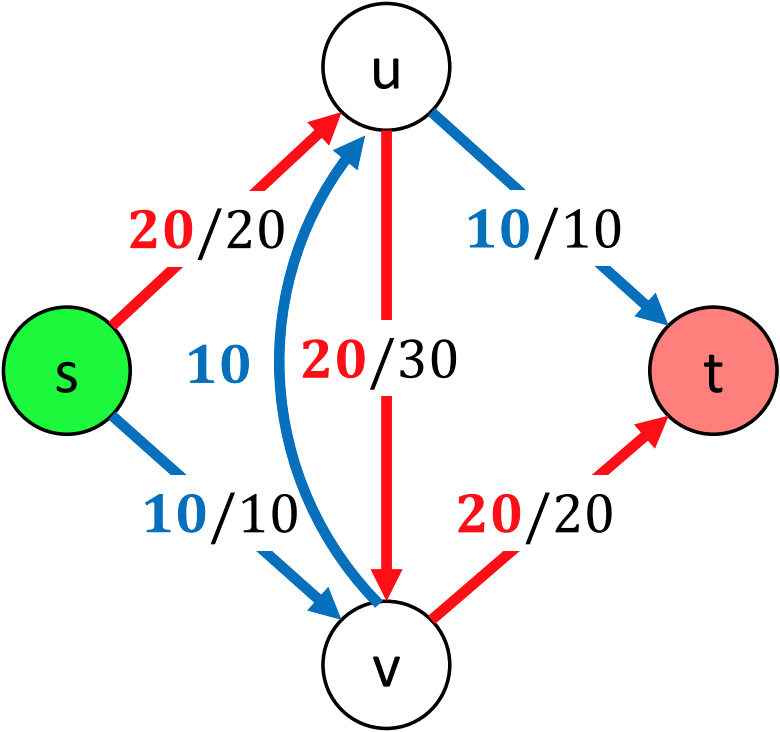
\includegraphics[width=0.25\linewidth]{figures/reverse-flow.png}
\end{figure}

\begin{definition}[Residual Graph]\index{Residual Graph}\label{def:residual-graph}
    Given a flow $f$ in a network $G = (V, E)$, the \term{residual graph} $G_f = (V, E_f)$ is a graph with the \bred{same vertices} as $G$, and edges $E_f$ defined as follows:
    \begin{itemize}
        \item \textbf{Forward edges:} $e = (u, v)$ with capacity $c(e) - f(e)$
        
        This is the amount of additional flow that can be sent along edge $e$.

        \item \textbf{Reverse edges:} $e^{rev} = (v, u)$ with capacity $f(e)$
        
        This is the amount of flow that can be sent backwards along edge $e$.
    \end{itemize}
\end{definition}

\begin{figure}[ht!]
    \centering
    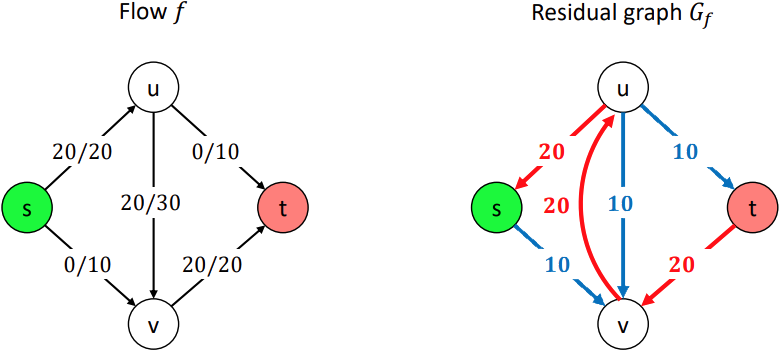
\includegraphics[width=0.63\linewidth]{figures/residual-graph.png}
\end{figure}

\begin{definition}[Augmenting Path]\index{Augmenting Path}\label{def:augmenting-path}
    Let $P$ be an $s-t$ path in the residual graph $G_f$. 

    Let $\text{bottleneck}(P, f)$ be the minimum capacity across all edges in $P$. 

    We \term{augment} flow $d$ by sending $\text{bottleneck}(P, f)$ units of flow along $P$. 

    \begin{itemize}
        \item For each forward edge $e \in P$, increase the flow on $e$ by $x$. 
        \item For each reverse edge $e^{rev} \in P$, decrease the flow on $e$ by $x$. 
    \end{itemize}
\end{definition}

\begin{figure}[ht!]
    \centering
    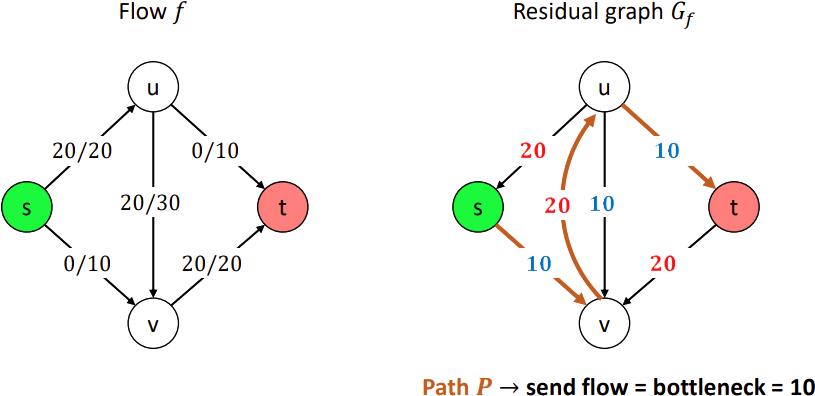
\includegraphics[width=0.65\linewidth]{figures/augmenting-path-1.png}
    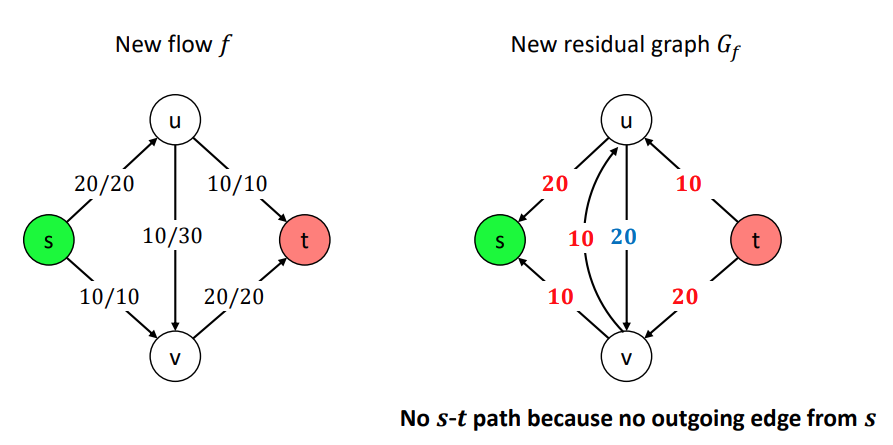
\includegraphics[width=0.65\linewidth]{figures/augmenting-path-2.png}
\end{figure}

We argue that the new flow is a valid flow. 

\begin{itemize}
    \item \textbf{Capacity constraint:} 
    
    \begin{itemize}
        \item If we \bred{increase} the flow on a forward edge, we can do so by \itblue{at most the capacity of forward edge} $e$ in $G_f$, which is $c(e) - f(e)$.
        
        So, the new flow can be at most $f(e) + \left( c(e) - f(e) \right) = c(e)$.

        \item If we \bred{decrease} the flow on a reverse edge, we can do so by \itblue{at most the capacity of reverse edge} $e^{rev}$ in $G_f$, which is $f(e)$.
        
        So, the new flow can be at most $f(e) - f(e) = 0$.
    \end{itemize}

    \item \textbf{Flow conservation:}

    Each node on the path (except $s$ and $t$) has exactly two incident edges. 

    \begin{center}
        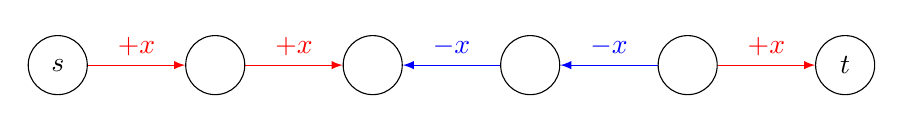
\begin{tikzpicture}
            \node[draw,circle,minimum size=0.75cm] (s) at (0, 0) {$s$};
            \node[draw,circle,minimum size=0.75cm] (1) at (2, 0) {};
            \node[draw,circle,minimum size=0.75cm] (2) at (4, 0) {};
            \node[draw,circle,minimum size=0.75cm] (3) at (6, 0) {};
            \node[draw,circle,minimum size=0.75cm] (4) at (8, 0) {};
            \node[draw,circle,minimum size=0.75cm] (t) at (10, 0) {$t$};

            \draw[-latex,red]  (s) -- (1) node[midway, above] {$+x$};
            \draw[-latex,red]  (1) -- (2) node[midway, above] {$+x$};
            \draw[-latex,blue] (3) -- (2) node[midway, above] {$-x$};
            \draw[-latex,blue] (4) -- (3) node[midway, above] {$-x$};
            \draw[-latex,red]  (4) -- (t) node[midway, above] {$+x$};
        \end{tikzpicture}
    \end{center}

    \begin{itemize}
        \item Both are forward / reverse edges. Then, one edge is incoming, and the other is outgoing.

        The flow is increased / decreased by the same amount.

        \begin{figure}[ht!]
            \centering
            \begin{subfigure}{0.45\linewidth}
                \centering
                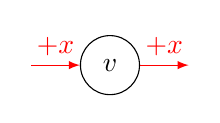
\begin{tikzpicture}
                    \node[draw,circle,minimum size=0.75cm] (v) at (0, 0) {$v$};

                    \draw[-latex,red] ++(180:1) -- (v)     node[midway, above] {$+x$};
                    \draw[-latex,red] (v)       -- ++(0:1) node[midway, above] {$+x$};
                \end{tikzpicture}

                \caption*{$f^{in}(v) \to +x \quad \text{and} \quad f^{out}(v) \to +x$}
            \end{subfigure}
            \hfil%
            \begin{subfigure}{0.45\linewidth}
                \centering
                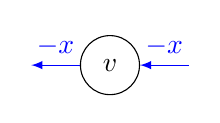
\begin{tikzpicture}
                    \node[draw,circle,minimum size=0.75cm] (v) at (0, 0) {$v$};

                    \draw[-latex,blue] (v)     -- ++(180:1) node[midway, above] {$-x$};
                    \draw[-latex,blue] ++(0:1) -- (v)       node[midway, above] {$-x$};
                \end{tikzpicture}

                \caption*{$f^{in}(v) \to -x \quad \text{and} \quad f^{out}(v) \to -x$}
            \end{subfigure}
        \end{figure}

        \item One forward, one reverse edge. Then, both edges are incoming or outgoing.

        The flow is increased on one edge and decreased on the other by the same amount.

        \begin{figure}[ht!]
            \begin{subfigure}{0.45\linewidth}
                \centering
                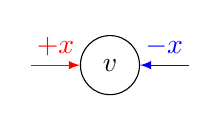
\begin{tikzpicture}
                    \node[draw,circle,minimum size=0.75cm] (v) at (0, 0) {$v$};

                    \draw[-latex,red]  ++(180:1) -- (v) node[midway, above] {$+x$};
                    \draw[-latex,blue] ++(0:1)   -- (v) node[midway, above] {$-x$};
                \end{tikzpicture}

                \caption*{$f^{in}(v)$ and $f^{out}(v)$ are unchanged}
            \end{subfigure}
            \hfil%
            \begin{subfigure}{0.45\linewidth}
                \centering
                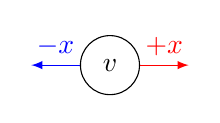
\begin{tikzpicture}
                    \node[draw,circle,minimum size=0.75cm] (v) at (0, 0) {$v$};

                    \draw[-latex,blue] (v) -- ++(180:1) node[midway, above] {$-x$};
                    \draw[-latex,red]  (v) -- ++(0:1)   node[midway, above] {$+x$};
                \end{tikzpicture}

                \caption*{$f^{in}(v)$ and $f^{out}(v)$ are unchanged}
            \end{subfigure}
        \end{figure}
    \end{itemize}
\end{itemize}

\section{Max Flow-Min Cut}

\subsection{Ford-Fulkerson Algorithm}

\begin{algorithm}[ht!]
    \begin{algorithmic}[1]
        \Function{Max-Flow}{$G$}
            \State {\color{gray} \texttt{// Initialize flow to 0:}}
            \State Set $f(e) = 0$ for all $e \in E$

            {~~~}

            \State {\color{gray} \texttt{// While there is an $s-t$ path in $G_f$:}}
            \While{$p = \Call{Find-Path}{s, t, \Call{Residual}{G,f}} \neq \texttt{None}$}
                \State $f \gets \Call{Augment}{f, p}$
                \State $\Call{Update-Residual}{G, f}$
            \EndWhile

            {~~~}

            \State \Return $f$
        \EndFunction
    \end{algorithmic}
\end{algorithm}

\subsubsection{Running Time Analysis}
\begin{itemize}
    \item \textbf{Number of Augmentations}
    
    \begin{itemize}
        \item At every step, flow and capacities remain integers. 
        \item For path $P$ in $G_f$, $\text{bottleneck}(P, f) > 0$ implies $\text{bottleneck}(P, f) \ge 1$.
        \item Each augmentation increases the flow by at least 1.
        \item The maximum flow (hence the number of augmentations) is at most $C = \sum_{e \text{ leaving } s} c(e)$.
    \end{itemize}

    \item \textbf{Preforming an Augmentation}
    
    \begin{itemize}
        \item $G_f$ has $n$ vertices and at most $2m$ edges. 
        \item Finding the path $P$, computing $\text{bottleneck}(P, f)$, and updating $G_f$ all take linear time. 
    \end{itemize}

    Thus, the running time of the Ford-Fulkerson algorithm is \[ O((m+n) \cdot C). \]
\end{itemize}

\subsubsection{Edmonds-Karp Algorithm}

This algorithm runs in \bred{pseudo-polynomial time} if we choose an \itblue{arbitrary} path in $G_f$ at each step. The value of $C$ can be exponentially larger in the input length (the number of bits requires to write down the edge capacities). 

\begin{example}
    In the graph below, we might end up repeatedly sending $1$ unit of flow across $a \to b$ and then reversing it. This takes $X$ steps, which can be exponential in the input length. 

    \begin{center}
        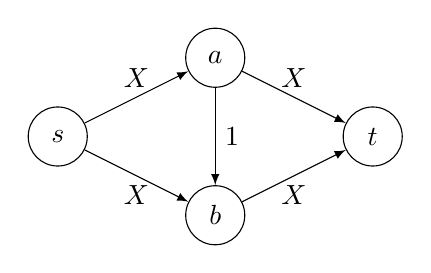
\begin{tikzpicture}
            \node[draw,circle,minimum size=0.75cm] (s) at (0, 0)  {$s$};
            \node[draw,circle,minimum size=0.75cm] (a) at (2, 1)  {$a$};
            \node[draw,circle,minimum size=0.75cm] (b) at (2, -1) {$b$};
            \node[draw,circle,minimum size=0.75cm] (t) at (4, 0)  {$t$};

            \draw[-latex] (s) -- (a) node[midway, above] {$X$};
            \draw[-latex] (s) -- (b) node[midway, below] {$X$};
            \draw[-latex] (a) -- (t) node[midway, above] {$X$};
            \draw[-latex] (b) -- (t) node[midway, below] {$X$};
            \draw[-latex] (a) -- (b) node[midway, right] {$1$};
        \end{tikzpicture}
    \end{center}
\end{example}

\begin{remark}[Pesudo-polynomial, Weakly Polynomial, and Strongly Polynomial]
    \begin{itemize}
        \item \textbf{Pseudo-polynomial time:} 
        
        The running time is polynomial in the unary representation of the input, \[
            ops = poly(m, n, X).
        \]

        \item \textbf{Weakly Polynomial time:} 
        
        The running time is polynomial in the binary representation of the input, \[
            ops = poly(m, n, \log X).
        \]

        \item \textbf{Strong polynomial time:} 
        
        The running time is polynomial in the input length, \[
            ops = poly(m, n).
        \]
    \end{itemize}
\end{remark}

To avoid the exponential running time, we need to be more careful about the path we choose. 

\begin{itemize}
    \item Find the \bred{maximum bottleneck capacity} augmenting path 
    
    This makes the algorithm run in \itblue{weakly polynomial time} \[
        \mathcal{O}(m^2 \cdot \log C)
    \]

    \item Find the \bred{shortest augmenting path} using BFS 
    
    This makes the algorithm run in \itblue{strongly polynomial time} \[
        \mathcal{O}(m^2 \cdot n).
    \] This is known as the \bred{Edmonds-Karp algorithm}\index{Edmonds-Karp Algorithm}.

    \begin{algorithm}[ht!]
        \begin{algorithmic}[1]
            \Function{Edmonds-Karp}{$G$}
                \State {\color{gray} \texttt{// Initialize flow to 0:}}
                \State Set $f(e) = 0$ for all $e \in E$

                {~~~}

                \State {\color{gray} \texttt{// Find shortest $s-t$ path in $G_f$:}}
                \While{$p = \Call{BFS}{s, t, \Call{Residual}{G,f}} \neq \texttt{None}$}
                    \State $f \gets \Call{Augment}{f, p}$
                    \State $\Call{Update-Residual}{G, f}$
                \EndWhile

                {~~~}

                \State \Return $f$
            \EndFunction
        \end{algorithmic}
    \end{algorithm}
    
    \begin{proof}
        Proof of \textsc{Edmonds-Karp} algorithm running time. 

        Let $d(v)$ be the distance from $s$ to $v$ in the residual graph $G_f$.

        \begin{lemma*}[1]\label{lem:edmonds-karp-1}
            During the execution of the algorithm, $d(v)$ does not decrease for any $v$.
        \end{lemma*}

        \begin{proof}(\hyperref[lem:edmonds-karp-1]{Lemma 1})

            Suppose augmentation $f \to f'$ decreases $d(v)$ for some $v$.

            Choose the $v$ with the smallest $d(v)$ in $G_{f'}$.

            Say $d(v) = k$ in $G_{f'}$, so $d(v) \ge k + 1$ in $G_f$.

            We look at node $u$ just before $v$ on a shortest path $s \to v \in G_{f'}$. 

            \begin{itemize}
                \item $d(u) = k - 1$ in $G_{f'}$
                \item $d(u)$ didn't decrease, so $d(u) \le k - 1$ in $G_f$.
            \end{itemize} 
            \[
                \begin{matrix}
                           & d(u)       & d(v)       \\
                    G_f    & \le k - 1  & \ge k + 1  \\
                           & \downarrow & \downarrow \\
                    G_{f'} & k - 1      & k
                \end{matrix}
            \]

            Then, in $G_f$, $(u, v)$ must be missing, as otherwise $d(v) \le d(u) + 1 = k$ in $G_f$.

            We must have added $(u, v)$ by selecting $(v, u)$ in augmenting path $P$.

            However, $P$ is a shortest path in $G_{f'}$, so it cannot have edge $(v, u)$ with $d(v) > d(u)$.
        \end{proof}

        We call edge $(u, v)$ \bred{critical} in an augmentation step if 
        \begin{itemize}
            \item It is part of the augmenting path $P$ and its capacity is equal to bottleneck$(P, f)$, or
            \item Augmentation step removes $e$ and adds $e^{rev}$ (if missing).
        \end{itemize}

        \begin{lemma*}[2]\label{lem:edmonds-karp-2}
            Between any two steps in which $(u, v)$ is critical, the distance $d(v)$ increases by at least 2.
        \end{lemma*}

        \begin{proof}(\hyperref[lem:edmonds-karp-2]{Lemma 2})
            
            Suppose $(u, v)$ was critical in $G_f$. The augmenting path must have removed it. 

            Let $k = d(u)$ in $G_f$. Since $(u, v)$ is part of a shortest path, $d(v) = k + 1$ in $G_f$.

            For $(u, v)$ to be critical again, it must be added back at some point. 
            \begin{itemize}
                \item Suppose $f' \to f''$ steps adds $(u, v)$ back.
                \item Augmenting path in $f'$ must have selected $(v, u)$.
                \item In $G_{f'}$, $d(v) = k + 1 \ge (k + 1) + 1 = k + 2$ by \hyperref[lem:edmonds-karp-1]{Lemma 1} on $v$.  \end{itemize}
        \end{proof}

        Each $d(u)$ can go from $0$ to $n$ by \hyperref[lem:edmonds-karp-1]{Lemma 1}.

        Then, each edge $(u, v)$ can be critical at most $\frac{n}{2}$ times by \hyperref[lem:edmonds-karp-2]{Lemme 2}.

        There can be at most $m \cdot \frac{n}{2}$ augmentation steps, and each augmentation takes $O(m)$ time.

        Thus, the running time of the Edmonds-Karp algorithm is \[
            O(m^2 \cdot n).
        \]
    \end{proof}
\end{itemize}

\subsection{Max Flow-Min Cut Theorem}

\begin{definition}[$s-t$ Cut]\index{$s-t$ Cut}\label{def:s-t-cut}
    An \term{$s-t$ cut} is a partition of the vertices $V = S \cup T$ such that $s \in S$ and $t \in T$.
\end{definition}

The capacity of an $s-t$ cut is the sum of the capacities of edges leaving $S$ and entering $T$ \[
    \text{cap}(S, T) = \sum_{u \in S} \sum_{v \in T} c(u, v)
\]

\begin{figure}[ht!]
    \centering
    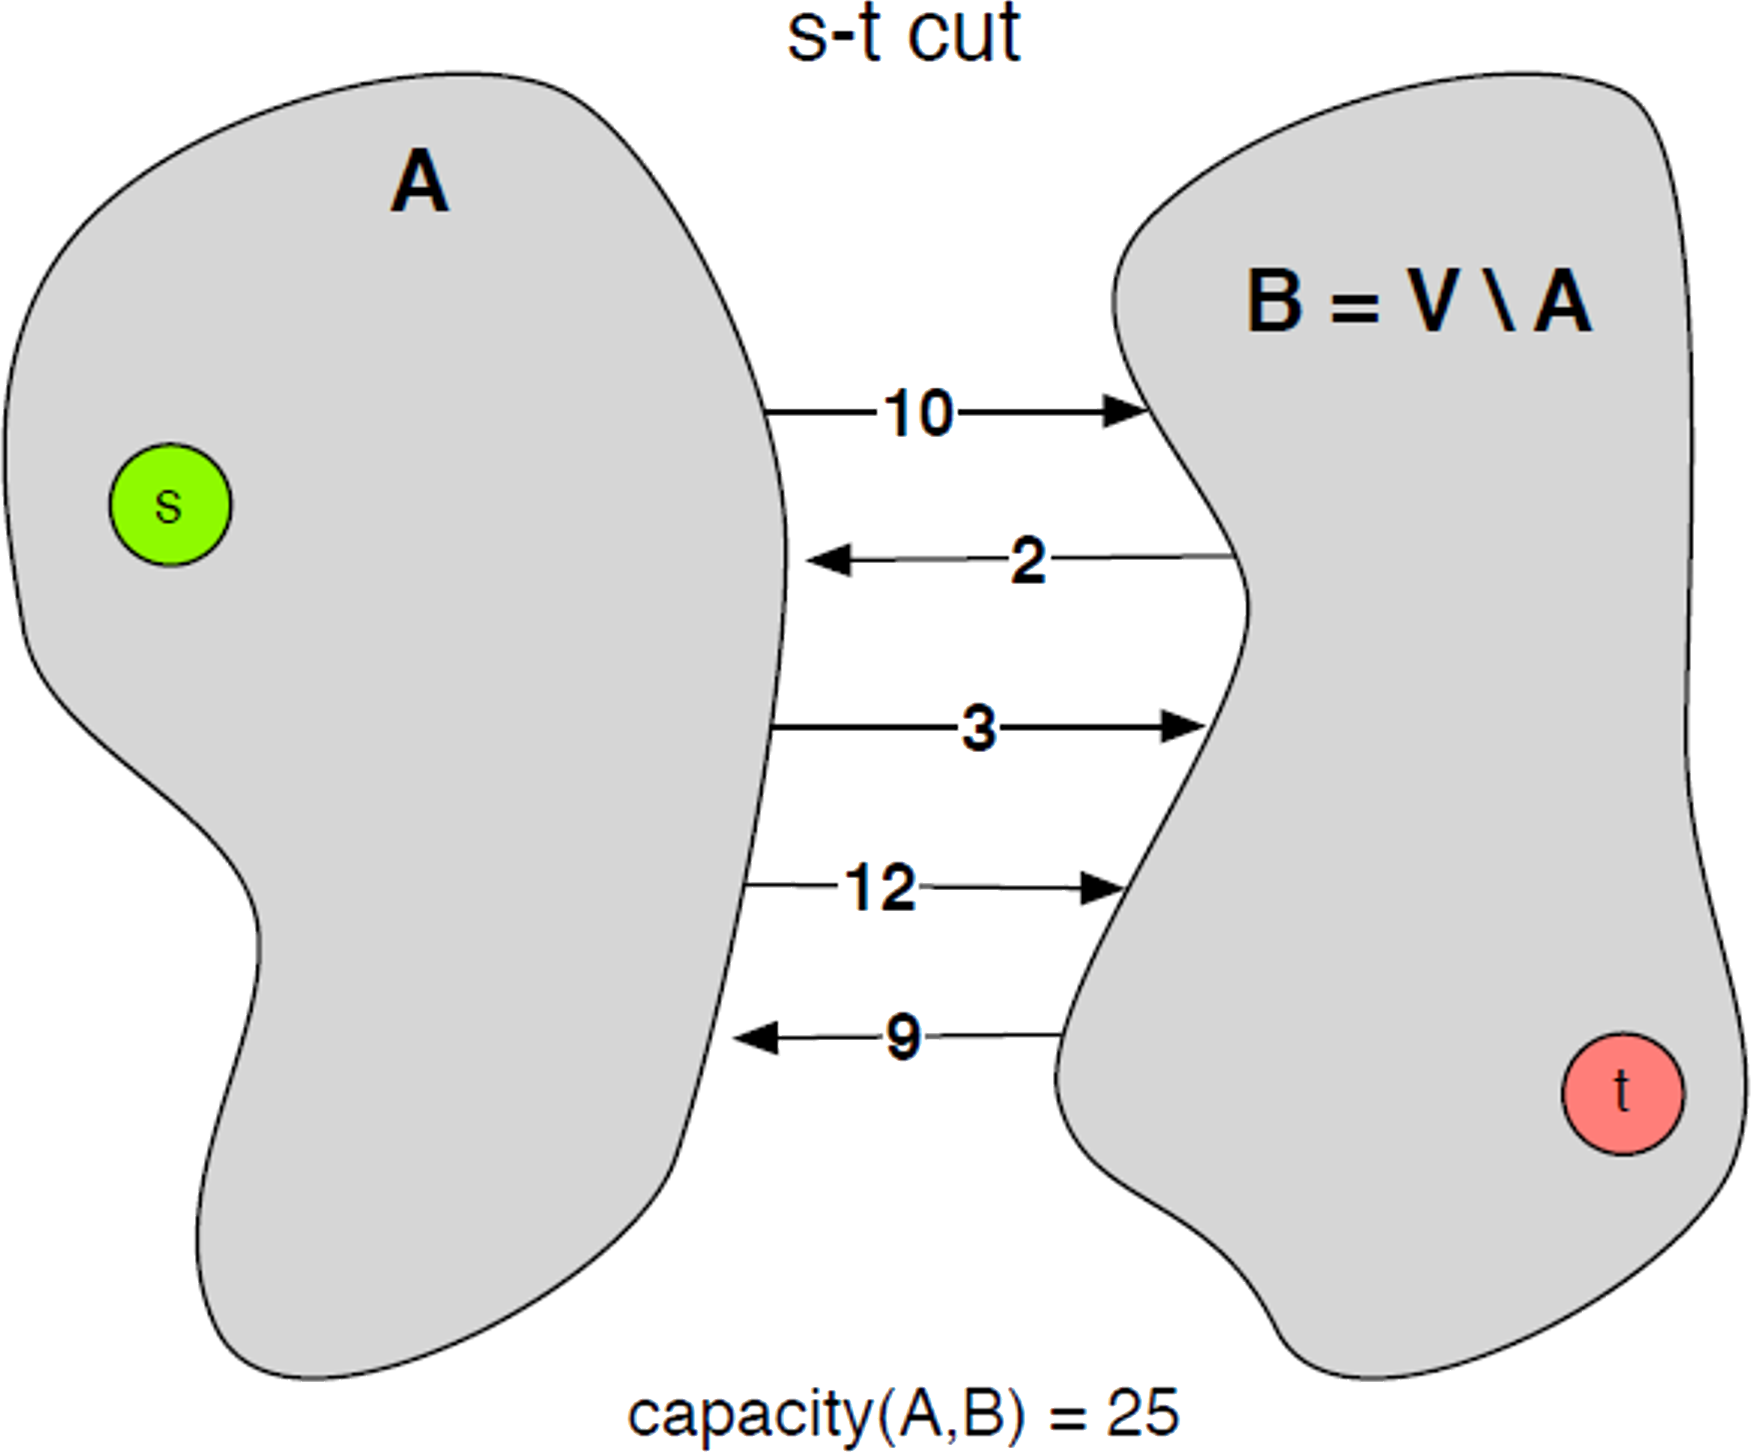
\includegraphics[width=0.33\linewidth]{figures/st-cut.png}
\end{figure}

\begin{theorem}
    For any flow $f$ and any $s-t$ cut $(S, T)$, \[
        v(f) = f^{out}(S) - f^{in}(S)
    \]
\end{theorem}

\begin{proof}
    Let $v \in S \setminus \{s\}$. Then,
    \begin{align*}
        f^{in}(v)
         & = f^{out}(v)                                                                     \\
        \sum_{v \in S \setminus \{s\}} \left( \sum_{e \text{ entering } v} f(e) \right)
         & = \sum_{v \in S \setminus \{s\}} \left( \sum_{e \text{ leaving } v} f(e) \right)
    \end{align*}

    After rearrangement, we get \[
        v(f) = f^{out}(S) - f^{in}(S)
    \]
\end{proof}

\begin{theorem}
    For any flow $f$, and any $s-t$ cut $(S, T)$, \[
        v(f) \le \text{cap}(S, T)
    \]
\end{theorem}

\begin{proof}
    \begin{align*}
        v(f) & = f^{out}(A) - f^{in}(A)             \\
             & \le f^{out}(A)                       \\
             & = \sum_{e \text{ leaving } A} f(e)   \\
             & \le \sum_{e \text{ leaving } A} c(e) \\
             & = \text{cap}(A, B)
    \end{align*}
\end{proof}

Hence, \[
    \max_{f} v(f) \le \min_{(S, T)} \text{cap}(S, T),
\] the maximum flow is at most the minimum cut.

\begin{theorem}
    Ford-Fulkerson algorithm finds a maximum flow $f^*$.
\end{theorem}

\begin{proof}
    WTS that the flow $f$ found by the Ford-Fulkerson algorithm is a maximum flow.

    Let $f$ be the flow found by the Ford-Fulkerson algorithm. 
    
    Let $G_f$ be the residual graph after the algorithm terminates.

    Let $A^*$ be the nodes reachable from $s$ in $G_f$, and let $B^* = V \setminus A^*$.

    \begin{center}
        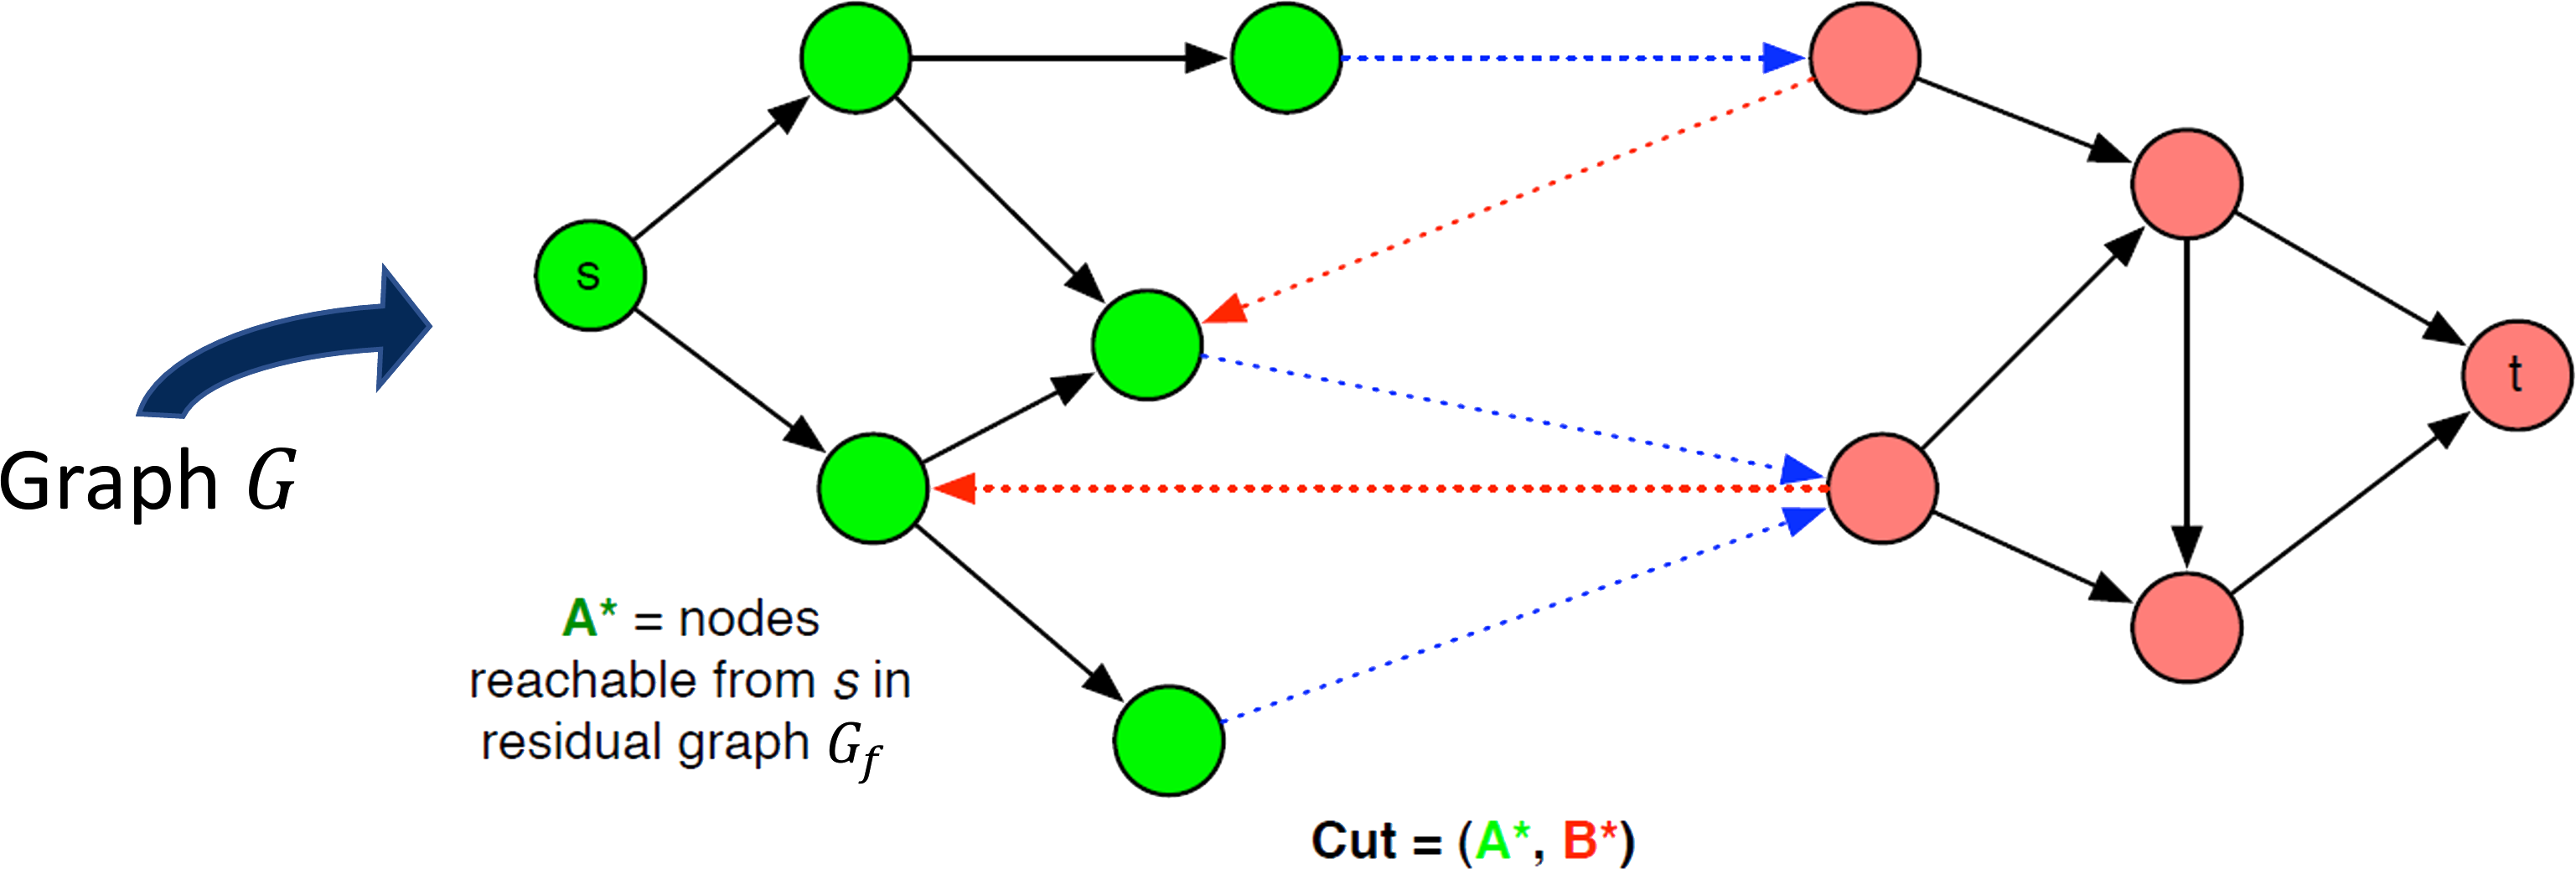
\includegraphics[width=0.67\linewidth]{figures/max-flow-min-cut.png}
    \end{center}

    \textbf{Claim:} $(A^*, B^*)$ is an $s-t$ cut.

    Indeed, $s \in A^*$ be definition. $t \in B^*$ because when Ford-Fulkerson terminates, there are no $s-t$ paths in $G_f$, so $s \notin A^*$. 

    {~~~}

    \begin{itemize}
        \item Let \blue{blue} edges be the edges going out of $A^*$ \bred{in $G$}, and 

        Each \blue{blue} edge $(u, v)$ must be saturated. 

        Otherwise, $G_f$ would have its forward edge $(u, v)$ and then $v \in A^*$. 

        Then, $f^{out}(A^*) = \text{cap}(A^*, B^*)$.

        \item Let \red{red} edges be the edges going out of $A^*$ \bred{in $G_f$}.

        Each \red{red} edge $(v, u)$ must have zero flow. 

        Otherwise, $G_f$ would have its reverse edge $(u, v)$ and then $v \in A^*$.

        Then, $f^{in}(A^*) = 0$.
    \end{itemize}

    Thus, \[
        v(f) = f^{out}(A^*) - f^{in}(A^*) = \text{cap}(A^*, B^*).
    \]
\end{proof}

\begin{theorem}[Max Flow-Min Cut Theorem]\index{Max Flow-Min Cut Theorem}
    In any flow network, the value of the maximum flow is equal to the capacity of the minimum cut.
\end{theorem}

\begin{proof}
    Run Ford-Fulkerson to find a max flow $f$. 

    Construct its residual graph $G_f$. 

    Le4t $A^*$ be the set of vertices reachable from $s$ in $G_f$.

    Then, $(A^*, V \setminus A^*)$ is a min $s-t$ cut.
\end{proof}

\section{Applications of Network Flow}

\subsection{Bipartite Matching}

\begin{definition}[Bipartite Graph]\index{Bipartite Graph}\label{def:bipartite-graph}
    A graph $G = (V, E)$ is \term{bipartite} if its vertex set $V$ can be partitioned into two sets $U$ and $V$ such that every edge in $E$ has one endpoint in $U$ and the other in $V$.
\end{definition}

A bipartite matching is when given a bipartite graph $G = (U \cup V, E)$, we want to find a maximum cardinality matching.

% TODO: Complete this section

\part{Appendices}

\chapter*{Bibliography}
\addcontentsline{toc}{part}{Bibliography}
\nocite{*}
\printbibliography[heading=bibempty]

\cleardoublepage
\phantomsection
\setlength{\columnsep}{0.75cm}
\addcontentsline{toc}{part}{Index}
\printindex

\end{document}